\documentclass[12pt,a4paper]{article}

\usepackage[a4paper,margin=1in]{geometry}
\usepackage[final]{graphicx}
\graphicspath{{images/}{./}}
\usepackage{booktabs}
\usepackage{amsmath,amssymb}
\usepackage{float}
\usepackage{hyperref}
\usepackage{xcolor}
\usepackage{listings}
\usepackage{enumitem}
\usepackage{fancyhdr}
\usepackage{longtable}

\hypersetup{colorlinks=true,linkcolor=blue,urlcolor=blue}

\pagestyle{fancy}
\fancyhf{}
\lhead{ICS1512}
\rhead{Machine Learning Algorithms Laboratory}
\cfoot{\thepage}

\lstset{
language=Python,
basicstyle=\ttfamily\small,
numbers=left,
frame=single,
breaklines=true,
showstringspaces=false
}

\begin{document}

% =====================================================================
% EXPERIMENT 1: IRIS FLOWER SPECIES CLASSIFICATION
% =====================================================================

\begin{tabular}{|p{4cm}|p{11cm}|}
\hline
Experiment No. & 1 \\ \hline
Experiment Title & Iris Flower Species Classification using Decision Tree, Logistic Regression and Feature Selection \textsuperscript{\href{https://github.com/arivuchezhiyan/Machine_Learning}{1}} \\ \hline
Student Name & Arivuchezhiyan E \\ \hline
Register Number & 3122247001006 \\ \hline
Faculty & Dr. Poreddy Ajay Kumar Reddy \\ \hline
Submission Date & 23/07/2026 \\ \hline
\end{tabular}

\section{Objective}
State the objective of the experiment:
In this lab, I built and evaluated two classification models, Decision Tree Classifier and Logistic Regression, using the Iris dataset. I also applied univariate feature selection using SelectKBest with the ANOVA F-test to identify key attributes and test if dropping less important features impacts overall accuracy.

\section{Problem Statement}
Describe the problem, input, output and objective:
The Iris task involves classifying flower species based on physical measurements.
\begin{itemize}
\item \textbf{Input}: 4 continuous feature columns representing sepal length (\texttt{SepalLengthCm}), sepal width (\texttt{SepalWidthCm}), petal length (\texttt{PetalLengthCm}) and petal width (\texttt{PetalWidthCm}).
\item \textbf{Output}: Species target label \texttt{Species} spanning 3 classes: Setosa (0), Versicolor (1) and Virginica (2).
\item \textbf{Objective}: Implement end-to-end data cleaning, exploratory analysis, label encoding, train-test splitting, feature selection, model training and performance evaluation.
\end{itemize}

\section{Dataset Description}
\begin{longtable}{|p{6cm}|p{8cm}|}
\hline
Dataset Name & Iris Dataset \\ \hline
Dataset Source & Iris.csv \\ \hline
Number of Samples & 150 \\ \hline
Number of Features & 4 (excluding ID column) \\ \hline
Number of Classes & 3 (Iris-setosa, Iris-versicolor Iris-virginica) \\ \hline
Missing Values & 0 missing values \\ \hline
Train-Test Split & 80\% Train (120 samples) / 20\% Test (30 samples) \\ \hline
\end{longtable}

\section{Exploratory Data Analysis}
Include all relevant visualizations:
\begin{itemize}
\item \textbf{Dataset overview}: The dataset contains 150 records, with 50 samples for each species. Every row records 4 numerical measurements in centimeters.
\item \textbf{Statistical summary}:
\begin{itemize}
\item Sepal Length: Ranges from 4.30 cm to 7.90 cm with a mean of 5.84 cm.
\item Sepal Width: Ranges from 2.00 cm to 4.40 cm with a mean of 3.05 cm.
\item Petal Length: Ranges from 1.00 cm to 6.90 cm with a mean of 3.76 cm.
\item Petal Width: Ranges from 0.10 cm to 2.50 cm with a mean of 1.20 cm.
\end{itemize}
\item \textbf{Missing value check}: Running \texttt{df.isnull().sum()} confirmed zero missing values across all columns.
\item \textbf{Class distribution}: The dataset is balanced with 50 entries each for Setosa, Versicolor and Virginica.
\item \textbf{Correlation analysis}: Petal length and petal width show a strong positive correlation ($r = 0.96$). Sepal length also correlates well with petal length ($r = 0.87$).
\item \textbf{Feature distribution}: Histograms display bimodal distributions for petal features, making them effective predictors.
\end{itemize}

\subsection*{Figure Template}

\begin{figure}[H]
\centering
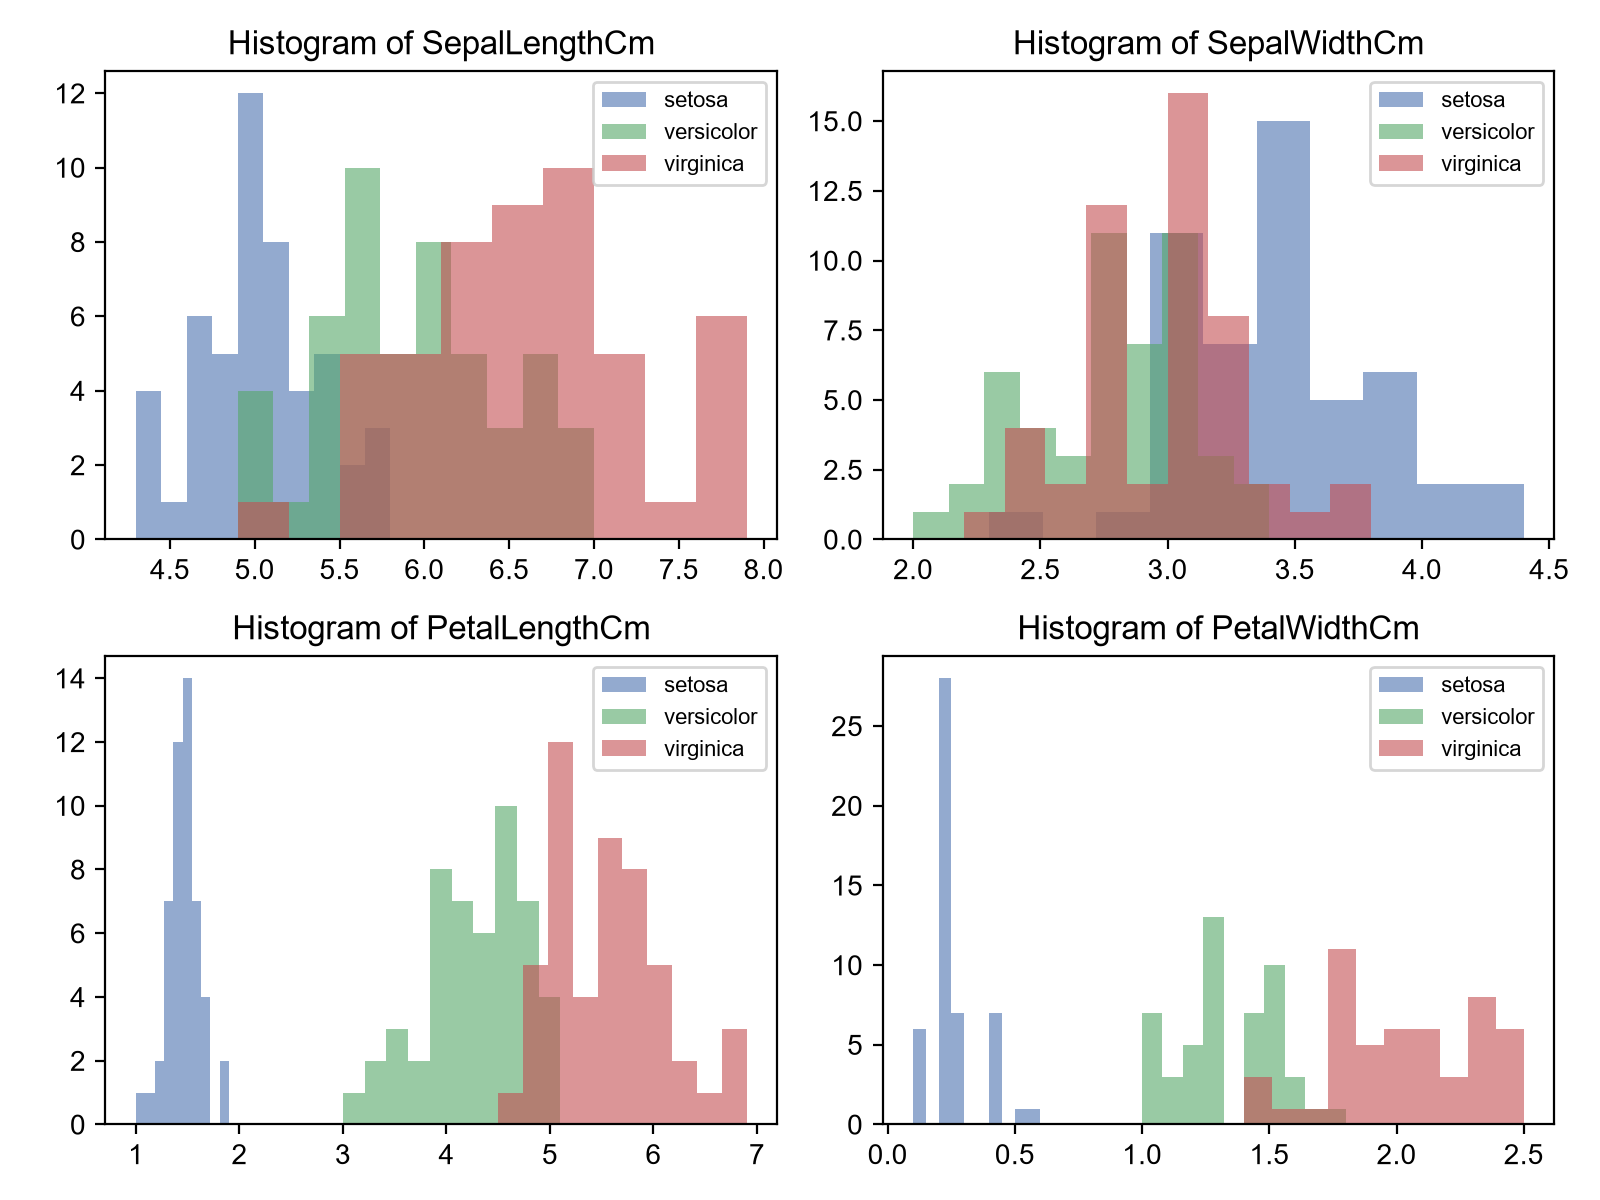
\includegraphics[width=0.7\linewidth]{iris_histograms.png}
\caption{Iris Dataset Feature Distributions (Histograms)}
\label{fig:exp1_iris_hist}
\end{figure}

\textbf{Inference:}
The feature histograms show distinct separated peaks for petal length and petal width. This indicates petal dimensions are far more effective for separating species than sepal measurements. Sepal width follows a typical bell curve centered around 3.0 cm.

\begin{figure}[H]
\centering
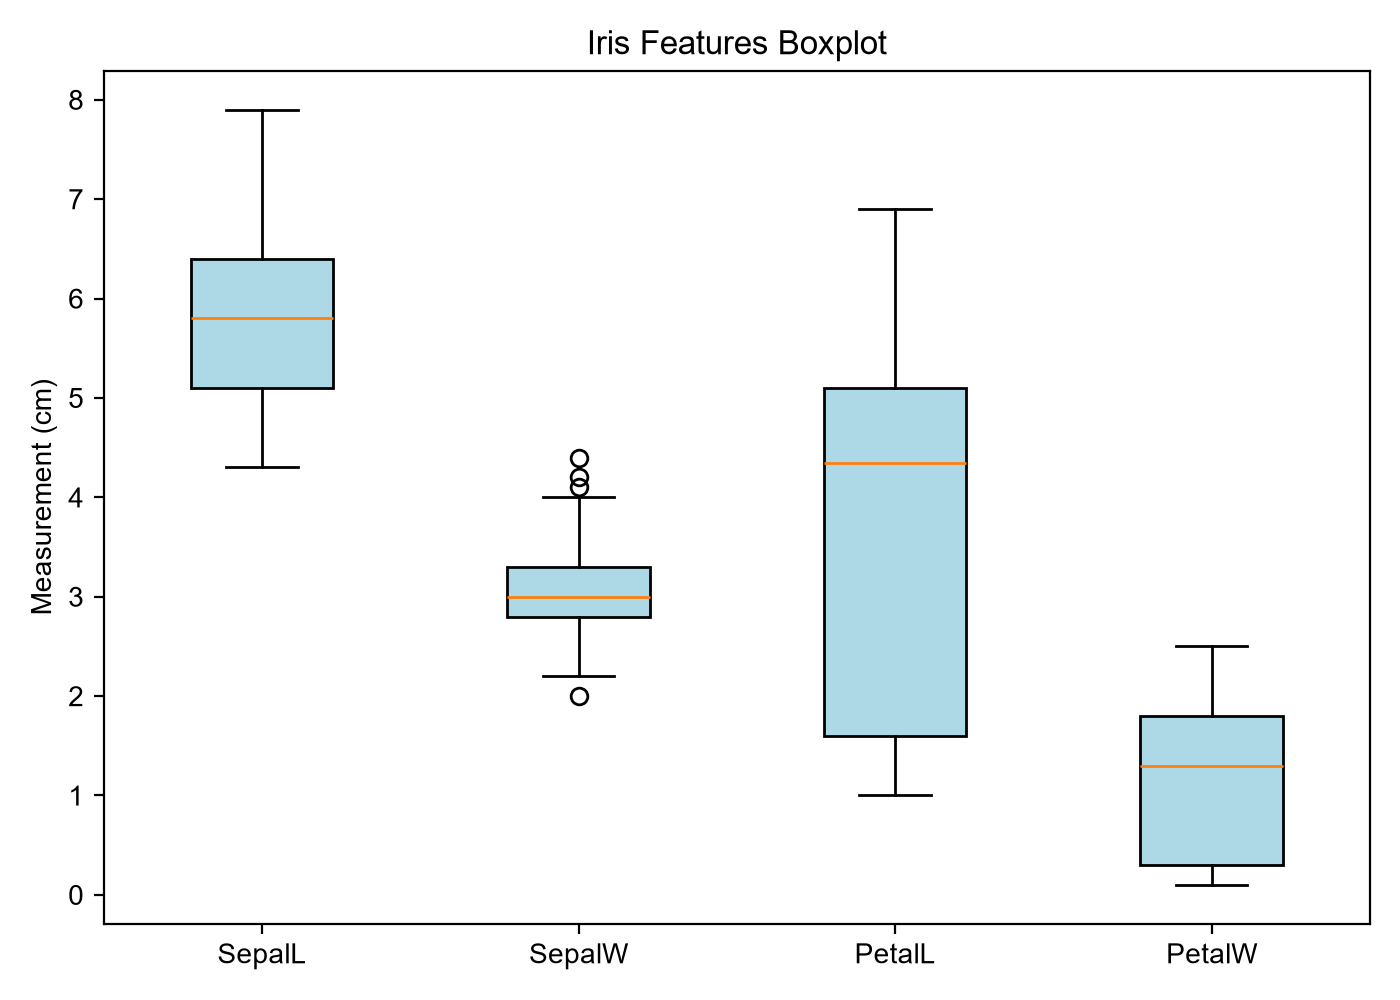
\includegraphics[width=0.7\linewidth]{iris_boxplot.png}
\caption{Iris Features Boxplot Analysis}
\label{fig:exp1_iris_box}
\end{figure}

\textbf{Inference:}
The boxplot illustrates the median and spread for each attribute. Sepal and petal lengths display wider ranges, while sepal width stays tightly grouped with a few minor outliers. Petal dimensions show clear separation between small and large values.

\begin{figure}[H]
\centering
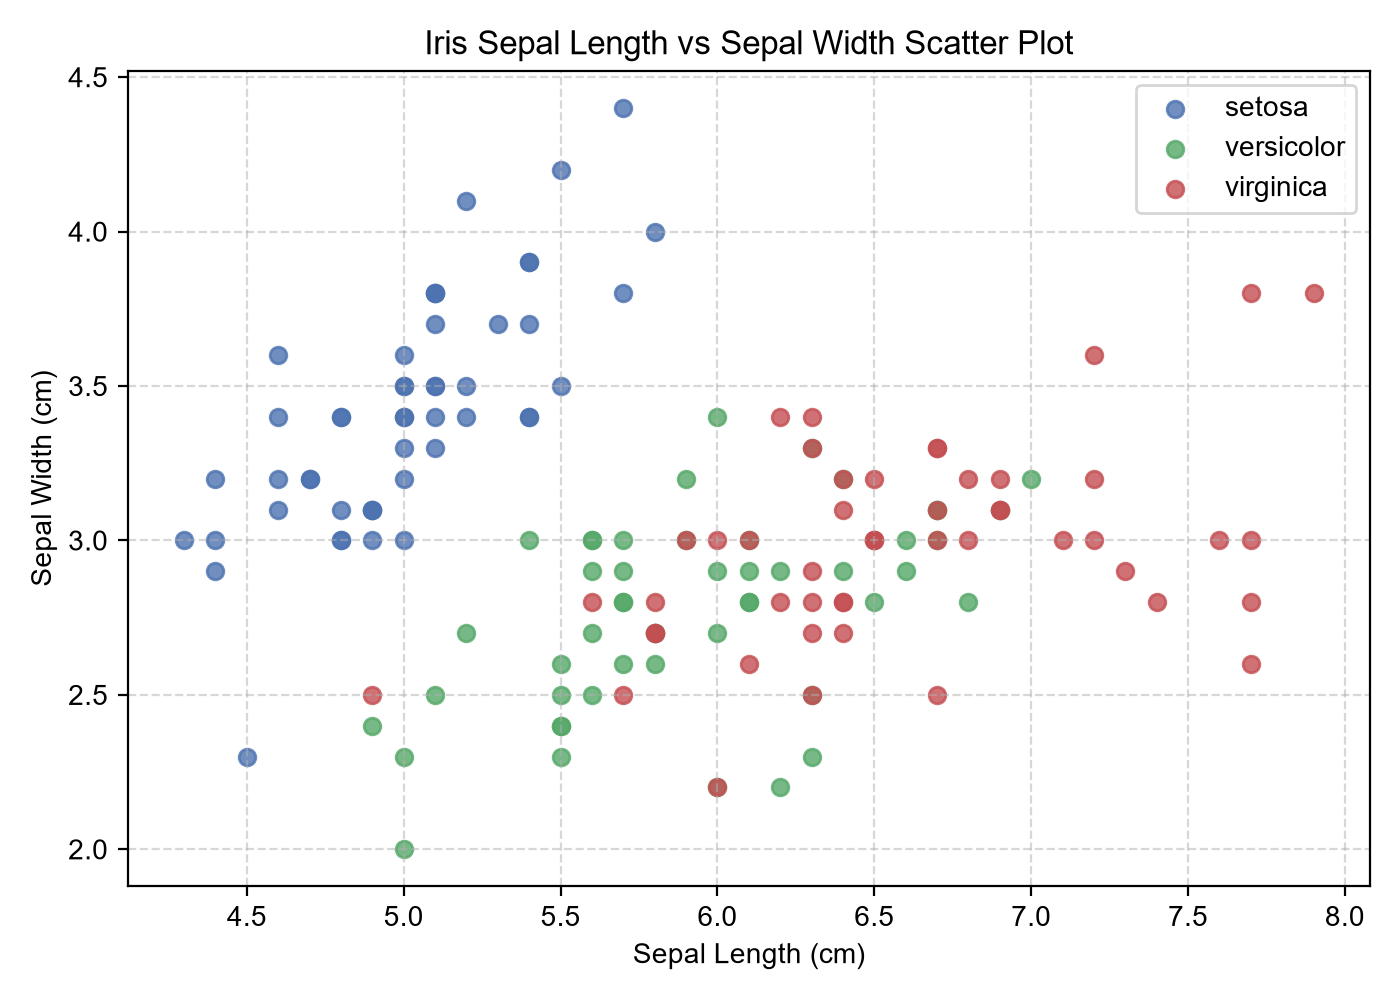
\includegraphics[width=0.7\linewidth]{iris_scatter.png}
\caption{Iris Sepal Length vs Sepal Width Scatter Plot}
\label{fig:exp1_iris_scatter}
\end{figure}

\textbf{Inference:}
Plotting sepal length against sepal width shows Setosa forming an isolated cluster at higher sepal widths. Versicolor and Virginica overlap considerably in sepal space, showing why sepal measurements alone are insufficient for classification.

\begin{figure}[H]
\centering
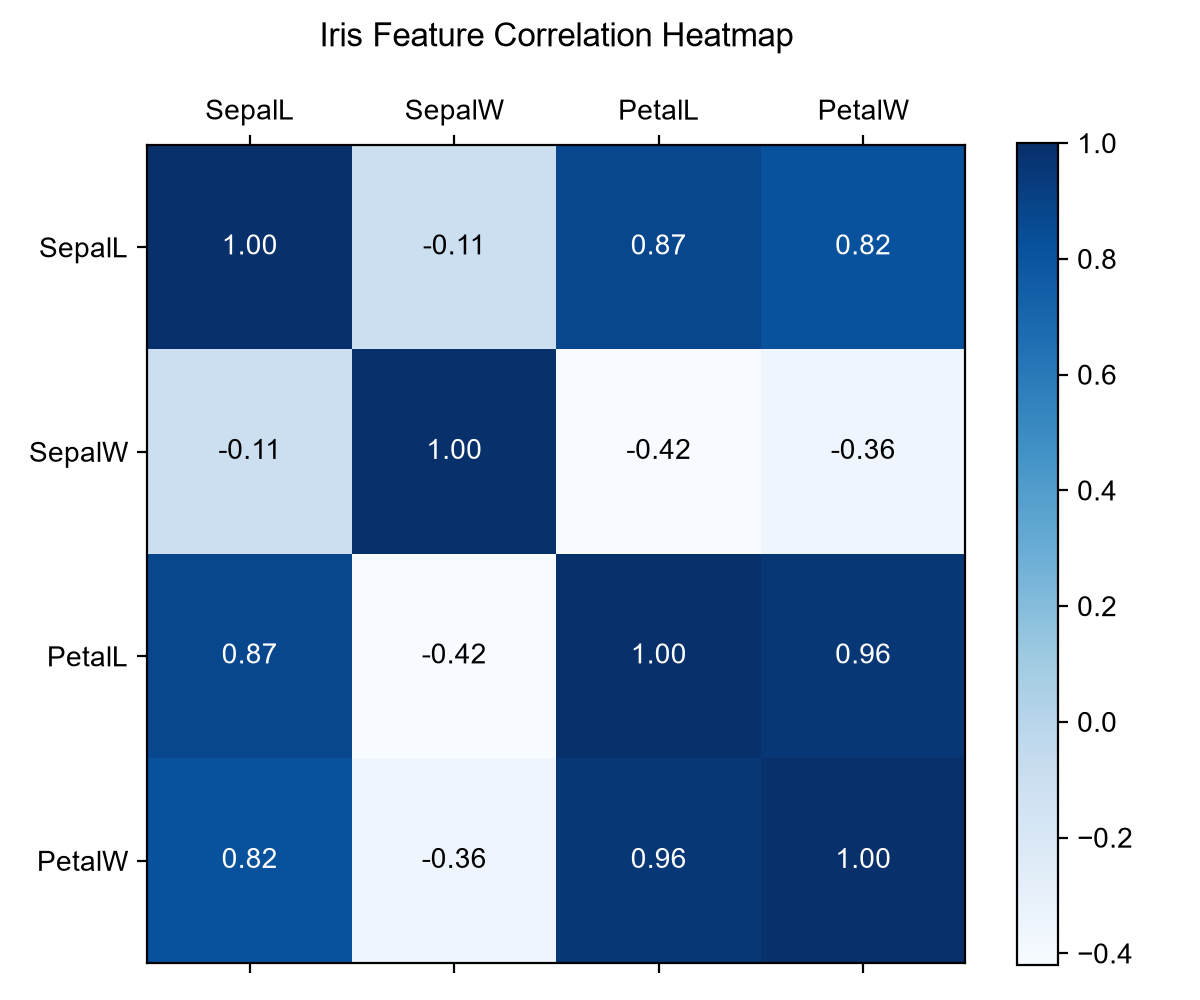
\includegraphics[width=0.7\linewidth]{iris_correlation.png}
\caption{Iris Correlation Matrix Heatmap}
\label{fig:exp1_iris_corr}
\end{figure}

\textbf{Inference:}
The correlation heatmap displays linear relationship strengths between features. Petal length and petal width show a strong positive correlation ($r \approx 0.96$). Sepal width correlates negatively with petal features, indicating feature redundancy where sepal columns can be dropped without losing performance.

\section{Data Preprocessing}

Explain:
\begin{itemize}
\item \textbf{Cleaning}: Checked for null values and dropped the unnecessary \texttt{Id} column.
\item \textbf{Label Encoding}: Converted species strings into integers using \texttt{LabelEncoder}: \texttt{Iris-setosa} $\rightarrow 0$, \texttt{Iris-versicolor} $\rightarrow 1$ and \texttt{Iris-virginica} $\rightarrow 2$.
\item \textbf{Train-test split}: Split data into 80\% training (120 samples) and 20\% testing (30 samples) using \texttt{random\_state=42}.
\item \textbf{Feature Selection}: Applied \texttt{SelectKBest} with ANOVA F-test ($f\_classif$) to select top 2 features. F-scores: \texttt{SepalLengthCm} (33.15), \texttt{SepalWidthCm} (23.36), \texttt{PetalLengthCm} (442.27) and \texttt{PetalWidthCm} (309.84). The selected top features were \texttt{PetalLengthCm} and \texttt{PetalWidthCm}.
\end{itemize}

\section{Machine Learning Algorithm}

Explain:
\begin{itemize}
\item \textbf{Decision Tree Classifier}:
\begin{itemize}
\item \textit{Working principle}: Splits feature space using decision boundaries to minimize Gini impurity at child nodes.
\item \textit{Math}: Gini Impurity $G = 1 - \sum_{k=1}^C p_k^2$. Information Gain measures impurity reduction.
\item \textit{Pros \& Cons}: Simple to interpret and visualize, but can overfit without depth constraints.
\end{itemize}
\item \textbf{Logistic Regression}:
\begin{itemize}
\item \textit{Working principle}: Computes class log-odds and outputs probabilities using multinomial softmax.
\item \textit{Math}: $P(y=k|\mathbf{x}) = \frac{e^{\mathbf{w}_k^T \mathbf{x}}}{\sum_j e^{\mathbf{w}_j^T \mathbf{x}}}$, optimized via cross-entropy loss.
\item \textit{Pros \& Cons}: Fast and outputs probabilities, but limited to linear boundaries.
\end{itemize}
\end{itemize}

\section{Experimental Setup}

\begin{tabular}{ll}
\toprule
Python Version & 3.13.0 \\
Scikit-Learn Version & 1.6.0 \\
IDE & Jupyter Notebook \\
Operating System & Windows 11 \\
Hardware & Intel Core i7 / 16 GB RAM \\
\bottomrule
\end{tabular}

\section{Hyperparameter Selection}

\begin{tabular}{ll}
\toprule
Parameter & Value\\
\midrule
DecisionTree criterion & Gini (default) \\
DecisionTree max\_depth & None (unconstrained) \\
DecisionTree random\_state & 42 \\
LogisticRegression solver & lbfgs (default) \\
LogisticRegression max\_iter & 1000 \\
SelectKBest k & 2 (score\_func=f\_classif) \\
Train-Test Split test\_size & 0.20 \\
Train-Test Split random\_state & 42 \\
\bottomrule
\end{tabular}

\section{Results}

\begin{tabular}{lc}
\toprule
Metric & Value\\
\midrule
Decision Tree Accuracy & 1.0000 (100\%) \\
Logistic Regression Accuracy & 1.0000 (100\%) \\
Precision (Macro Avg) & 1.00 \\
Recall (Macro Avg) & 1.00 \\
F1-score (Macro Avg) & 1.00 \\
\bottomrule
\end{tabular}

\subsection*{Detailed Classification Report and Confusion Matrix}

Confusion Matrix (Logistic Regression on Test Split):
\begin{equation*}
\begin{bmatrix}
10 & 0 & 0 \\
0 & 9 & 0 \\
0 & 0 & 11
\end{bmatrix}
\end{equation*}

Classification Report:
\begin{tabular}{lcccc}
\toprule
Class & Precision & Recall & F1-score & Support \\
\midrule
0 (Iris-setosa) & 1.00 & 1.00 & 1.00 & 10 \\
1 (Iris-versicolor) & 1.00 & 1.00 & 1.00 & 9 \\
2 (Iris-virginica) & 1.00 & 1.00 & 1.00 & 11 \\
\midrule
Accuracy & & & 1.00 & 30 \\
Macro Avg & 1.00 & 1.00 & 1.00 & 30 \\
Weighted Avg & 1.00 & 1.00 & 1.00 & 30 \\
\bottomrule
\end{tabular}

\section{Result Visualization}

Include all graphs generated during the experiment.

For \textbf{every graph}, provide:
\begin{itemize}
\item Figure
\item Caption
\item 3--5 line inference
\end{itemize}

Recommended figures:
\begin{enumerate}
\item Correlation Matrix
\item Class Distribution
\item Confusion Matrix
\item ROC Curve
\item Precision-Recall Curve
\item Learning Curve (if applicable)
\item Feature Importance (if applicable)
\end{enumerate}

\begin{figure}[H]
\centering
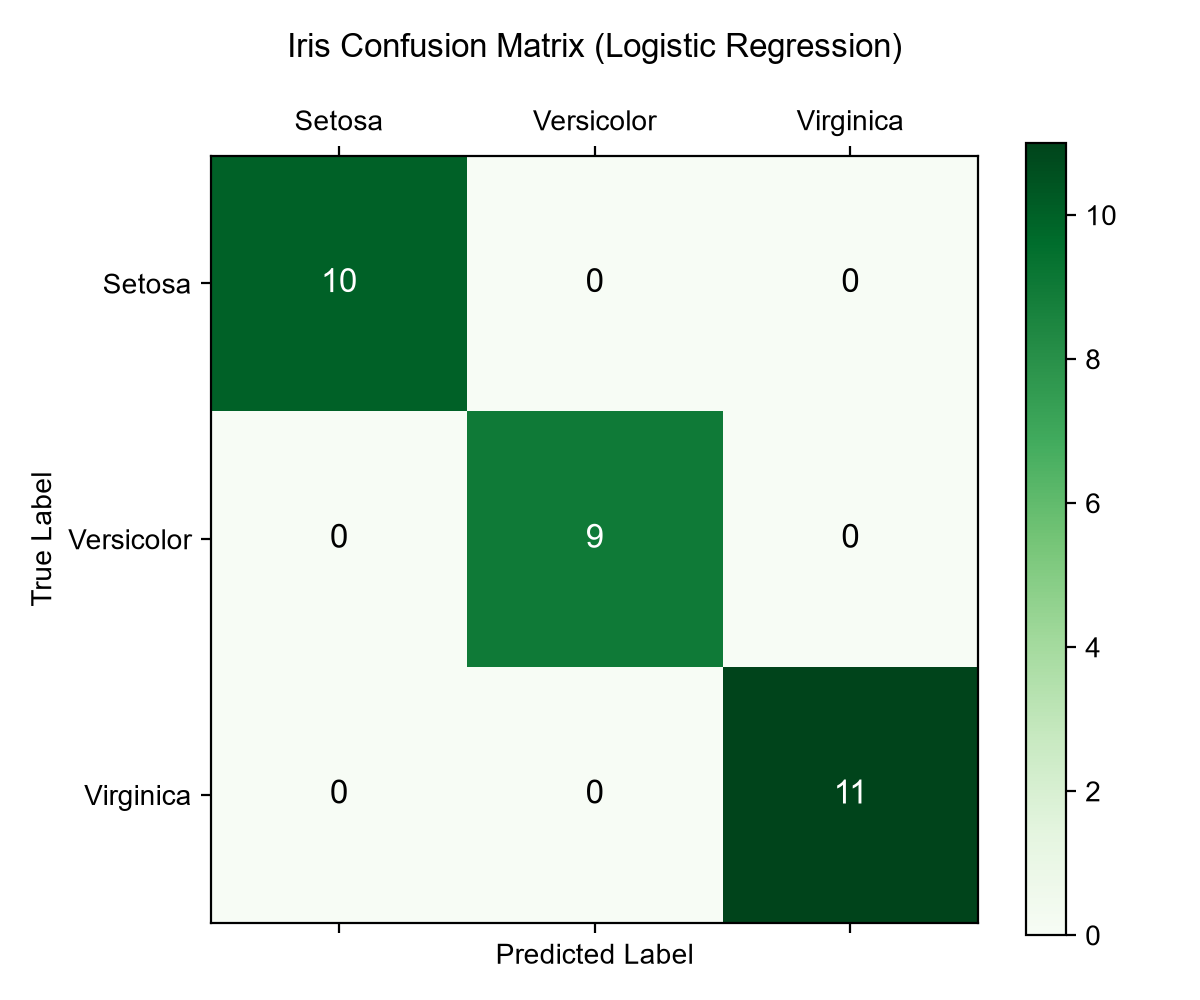
\includegraphics[width=0.7\linewidth]{iris_confusion_matrix.png}
\caption{Iris Dataset Confusion Matrix Heatmap}
\label{fig:exp1_iris_cm}
\end{figure}

\textbf{Inference:}
The confusion matrix shows zero misclassifications across all 30 test samples (10 Setosa, 9 Versicolor and 11 Virginica). Both models reached 100\% test accuracy, proving linear and tree-based methods separate the dataset effectively using all features or top petal attributes.

\section{Discussion}
Discuss observations, strengths, limitations and improvements:
\begin{enumerate}
\item \textbf{Class Separability}: The Iris dataset is easy to separate, with Setosa forming an isolated cluster away from other species.
\item \textbf{Model Performance}: Both models achieved 100\% accuracy, showing simple classifiers suit this problem well.
\item \textbf{Feature Importance}: ANOVA F-test scores confirmed petal length ($F=442.27$) and petal width ($F=309.84$) drive predictions.
\item \textbf{Limitations}: Small sample size (150 rows) means testing on larger datasets would provide stronger real-world validation.
\end{enumerate}

\section{Conclusion}
Summarize the experiment and key findings:
Decision Tree and Logistic Regression models both achieved 100\% accuracy on the Iris dataset. Using \texttt{SelectKBest} proved that 2 petal features provide the same accuracy as using all 4 attributes.

\section{References}
Use IEEE style:
\begin{enumerate}[label={[\arabic*]}]
\item F. Pedregosa \textit{et al.}, ``Scikit-learn: Machine learning in Python,'' \textit{Journal of Machine Learning Research}, vol. 12, pp. 2825--2830, 2011.
\item R. A. Fisher, ``The use of multiple measurements in taxonomic problems,'' \textit{Annals of Eugenics}, vol. 7, no. 2, pp. 179--188, 1936.
\end{enumerate}

\newpage

\newpage

% =====================================================================
% EXPERIMENT 2: SPAMBASE CLASSIFICATION & HYPERPARAMETER TUNING
% =====================================================================

\begin{tabular}{|p{4cm}|p{11cm}|}
\hline
Experiment No. & 2 \\ \hline
Experiment Title & Spambase Email Classification using Naive Bayes, K-Nearest Neighbors, Hyperparameter Tuning and Cross-Validation \textsuperscript{\href{https://github.com/arivuchezhiyan/Machine_Learning/tree/main/experiment_2}{2}} \\ \hline
Student Name & Arivuchezhiyan E \\ \hline
Register Number & 3122247001006 \\ \hline
Faculty & Dr. Poreddy Ajay Kumar Reddy \\ \hline
Submission Date & 23/07/2026 \\ \hline
\end{tabular}

\section{Objective}
State the objective of the experiment:
My main goal in this lab was testing different classification models on the Spambase dataset to see how well they filter spam emails. I built three types of Naive Bayes models (Gaussian, Multinomial and Bernoulli) along with a K-Nearest Neighbors model. To improve the KNN model performance I ran grid search and random search to pick optimal parameters. I also compared tree indexing methods like KDTree and BallTree and checked overall stability using 5-fold cross-validation.

\section{Problem Statement}
Describe the problem input output and objective:
Spam filtering involves classifying emails as either legitimate ham or unwanted spam based on key word and character counts.
\begin{itemize}
\item \textbf{Input}: 57 continuous attributes measuring word frequencies (\texttt{word\_freq\_*}) and character occurrences (\texttt{char\_freq\_*}).
\item \textbf{Output}: Target label \texttt{spam} (0 for ham and 1 for spam).
\item \textbf{Objective}: Normalize features with MinMaxScaler, split the data into 80\% train and 20\% test sets, fit Naive Bayes and KNN models, run hyperparameter tuning, plot ROC and PR curves and measure execution times.
\end{itemize}

\section{Dataset Description}
\begin{longtable}{|p{6cm}|p{8cm}|}
\hline
Dataset Name & Spambase Dataset \\ \hline
Dataset Source & spambase\_csv.csv \\ \hline
Number of Samples & 4601 \\ \hline
Number of Features & 57 continuous frequency features \\ \hline
Number of Classes & 2 (0: Ham [2788 samples], 1: Spam [1813 samples]) \\ \hline
Missing Values & 0 missing values \\ \hline
Train-Test Split & 80\% Train (3680 samples) / 20\% Test (921 samples) \\ \hline
\end{longtable}

\section{Exploratory Data Analysis}
Include all relevant visualizations:
\begin{itemize}
\item \textbf{Dataset overview}: The Spambase dataset contains 4601 rows with 57 numerical feature columns recording word frequencies.
\item \textbf{Class distribution}: There are 2788 ham emails (60.6\%) and 1813 spam emails (39.4\%).
\item \textbf{Missing value check}: Checking for missing entries with \texttt{df.isnull().sum()} showed no missing values anywhere.
\item \textbf{Feature scaling}: I scaled all feature values to the range between 0 and 1 using \texttt{MinMaxScaler}.
\end{itemize}

\subsection*{Figure Template}

\begin{figure}[H]
\centering
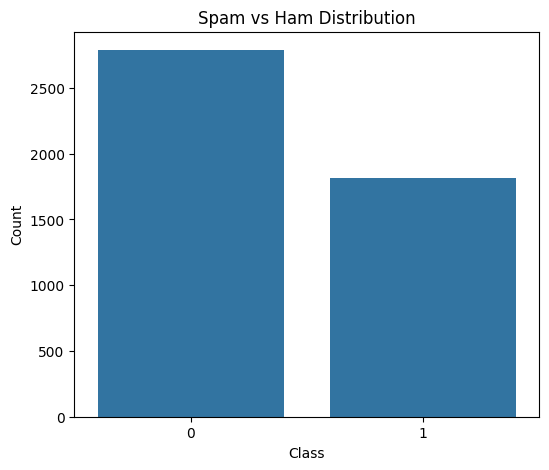
\includegraphics[width=0.6\linewidth]{spambase_class_distribution.png}
\caption{Spambase Target Class Distribution (Ham vs Spam)}
\label{fig:exp2_class_dist}
\end{figure}

\textbf{Inference:}
Looking at the class breakdown chart we have 2788 ham emails and 1813 spam emails. This moderate balance helps models learn patterns for both classes without getting biased toward one group.

\begin{figure}[H]
\centering
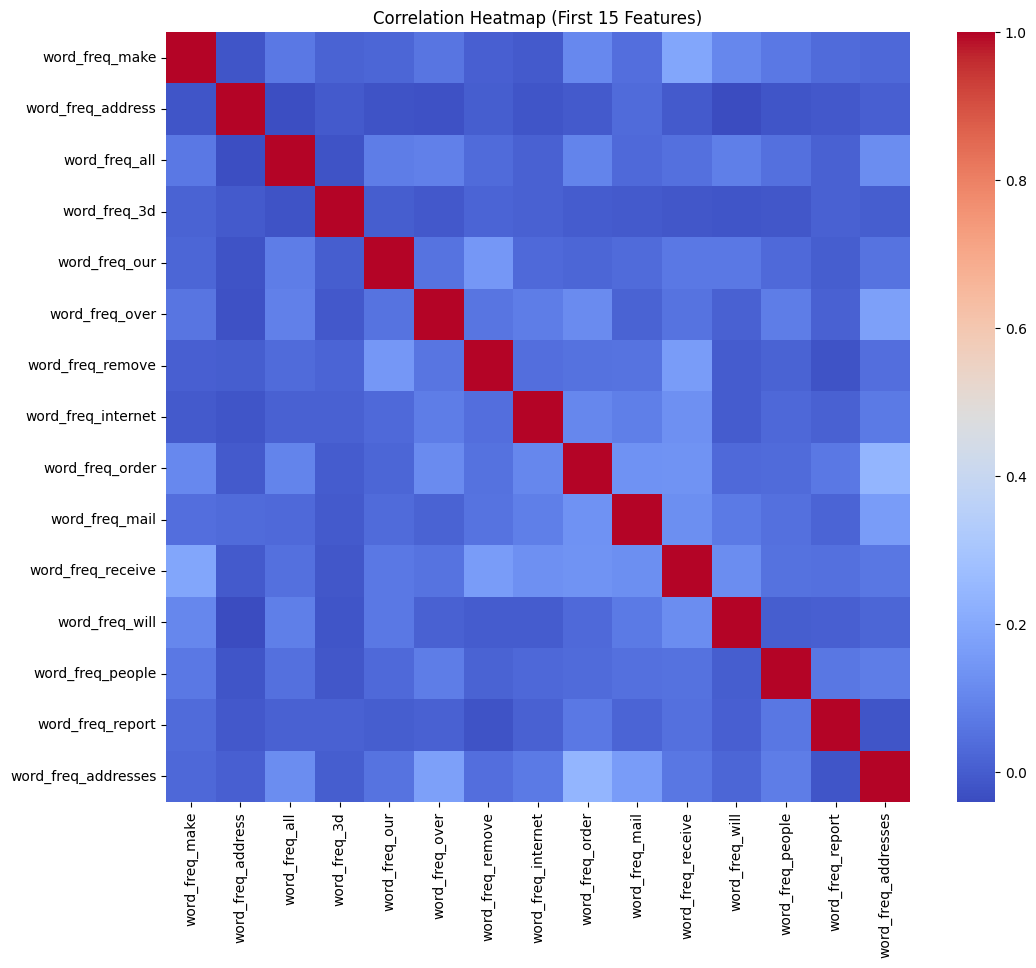
\includegraphics[width=0.75\linewidth]{spambase_correlation.png}
\caption{Spambase Correlation Heatmap (First 15 Features)}
\label{fig:exp2_corr}
\end{figure}

\textbf{Inference:}
The correlation plot for the first 15 features shows low linear correlation between columns. This supports the independence assumption used in Naive Bayes algorithms.

\begin{figure}[H]
\centering
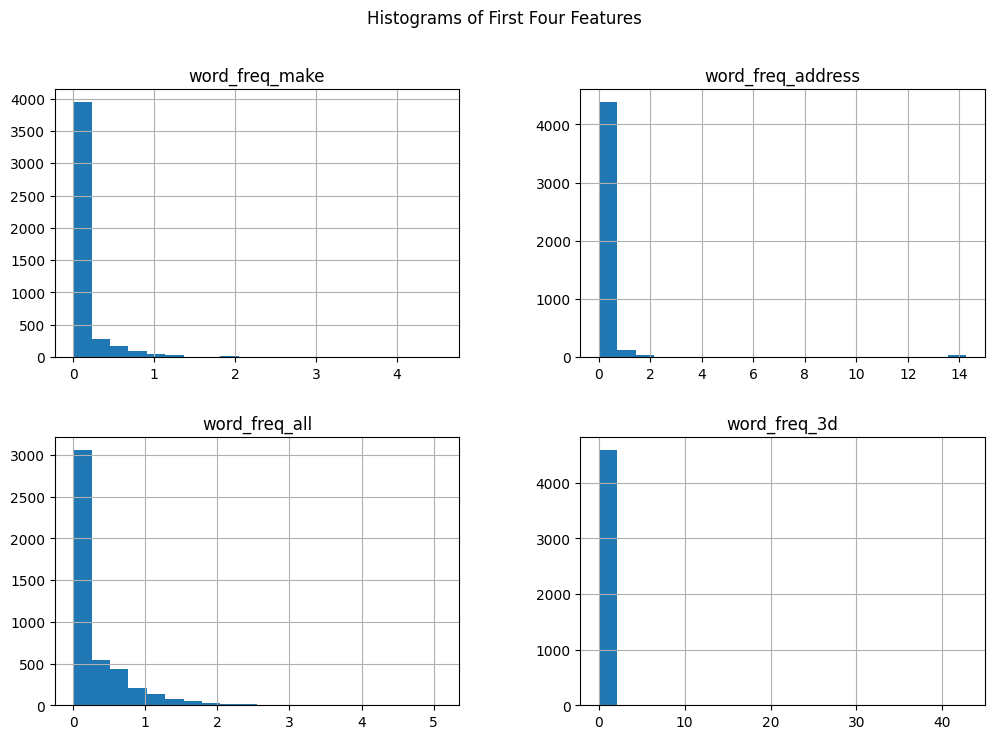
\includegraphics[width=0.75\linewidth]{spambase_histograms.png}
\caption{Histograms of First Four Word Frequency Features}
\label{fig:exp2_hist}
\end{figure}

\textbf{Inference:}
Histograms of word frequencies show a right skew. Most emails score zero for specific terms while spam messages show occasional high frequency spikes.

\begin{figure}[H]
\centering
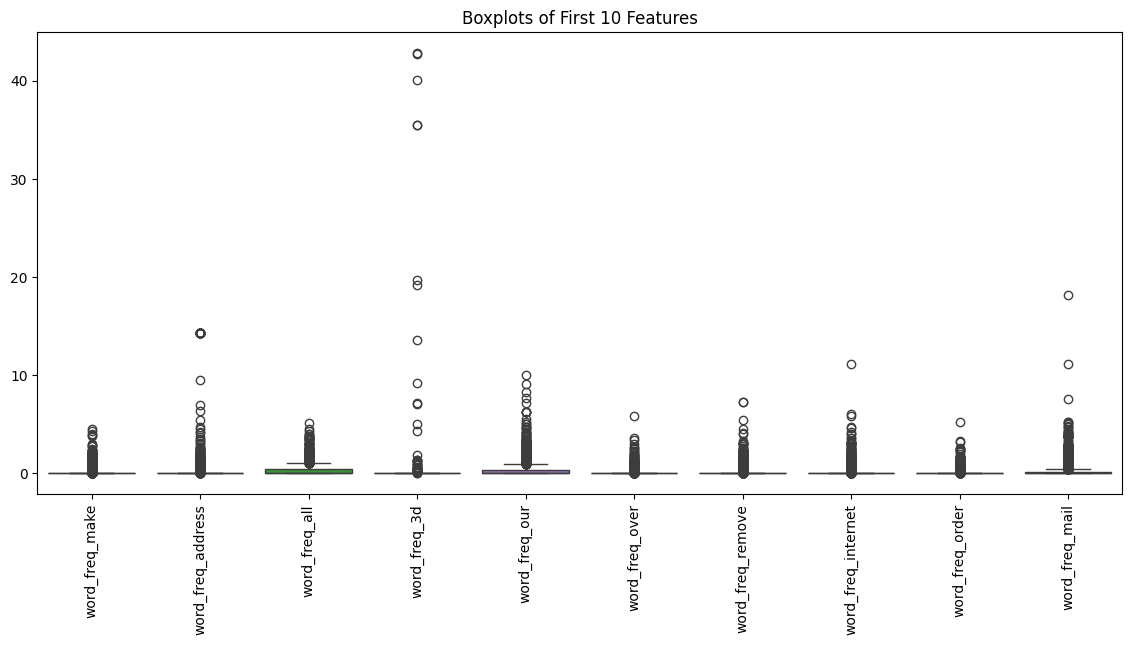
\includegraphics[width=0.85\linewidth]{spambase_boxplot.png}
\caption{Boxplots of First 10 Frequency Features}
\label{fig:exp2_box}
\end{figure}

\textbf{Inference:}
The boxplot displays low medians with several upper outliers. This confirms why scaling features with MinMaxScaler is important before running distance calculations in KNN.

\section{Data Preprocessing}

Explain:
\begin{itemize}
\item \textbf{Cleaning}: Checked dataset completeness using null check functions.
\item \textbf{Scaling}: Scaled numerical features into the range 0 to 1 with \texttt{MinMaxScaler}.
\item \textbf{Train-test split}: Split the dataset into 80\% training data and 20\% test data using stratified sampling.
\item \textbf{Binarization}: Created binary feature arrays using thresholding at 0.5 for Bernoulli Naive Bayes.
\end{itemize}

\section{Machine Learning Algorithm}

Explain:
\begin{itemize}
\item \textbf{Gaussian Naive Bayes}: Assumes features follow a normal distribution curve across classes $P(x_i|y) = \frac{1}{\sqrt{2\pi\sigma_y^2}} \exp\left(-\frac{(x_i-\mu_y)^2}{2\sigma_y^2}\right)$.
\item \textbf{Multinomial Naive Bayes}: Works well for word frequency counts by tracking term probabilities.
\item \textbf{Bernoulli Naive Bayes}: Handles binary inputs by checking whether key words are present or absent.
\item \textbf{K-Nearest Neighbors (KNN)}: Classifies test samples based on majority voting among k nearest neighbors using Euclidean and Manhattan distance metrics.
\item \textbf{GridSearchCV and RandomizedSearchCV}: Test different parameter combinations to find the best k value distance metric and neighbor weights.
\end{itemize}

\section{Experimental Setup}

\begin{tabular}{ll}
\toprule
Python Version & 3.13.0 \\
Scikit-Learn Version & 1.6.0 \\
IDE & Jupyter Notebook \\
Operating System & Windows 11 \\
Hardware & Intel Core i7 / 16 GB RAM \\
\bottomrule
\end{tabular}

\section{Hyperparameter Selection}

\begin{tabular}{ll}
\toprule
Parameter & Value\\
\midrule
Tested $k$ values & 1, 3, 5, 7, 9, 11 \\
Optimal $k$ (Baseline KNN) & 5 \\
GridSearchCV Parameter Space & $k \in [1..11]$, metrics: Euclidean/Manhattan, weights: uniform/distance \\
RandomizedSearchCV Parameter Space & $k \in [1..19]$, n\_iter: 20, cv: 5 \\
Cross-Validation Folds & 5-Fold Stratified K-Fold \\
MinMaxScaler Range & $[0, 1]$ \\
\bottomrule
\end{tabular}

\section{Results}

\subsection*{Naive Bayes Variant Comparison}
\begin{tabular}{lccccc}
\toprule
Model & Accuracy & Precision & Recall & F1-score & ROC-AUC \\
\midrule
Gaussian NB & 0.8328 & 0.7146 & 0.9587 & 0.8188 & 0.9229 \\
Multinomial NB & 0.8936 & 0.9431 & 0.7769 & 0.8520 & 0.9625 \\
Bernoulli NB & 0.6341 & 0.9643 & 0.0744 & 0.1381 & 0.5875 \\
\bottomrule
\end{tabular}

\subsection*{KNN Performance Across $k$ Values}
\begin{tabular}{ccccc}
\toprule
$k$ & Accuracy & Precision & Recall & F1-score \\
\midrule
1 & 0.8958 & 0.8678 & 0.8678 & 0.8678 \\
3 & 0.8958 & 0.8825 & 0.8485 & 0.8652 \\
\textbf{5} & \textbf{0.9023} & \textbf{0.8760} & \textbf{0.8760} & \textbf{0.8760} \\
7 & 0.8958 & 0.8761 & 0.8567 & 0.8663 \\
9 & 0.8947 & 0.8866 & 0.8402 & 0.8628 \\
11 & 0.8893 & 0.8851 & 0.8264 & 0.8547 \\
\bottomrule
\end{tabular}

\subsection*{Hyperparameter Search Optimization (GridSearchCV vs RandomizedSearchCV)}
\begin{tabular}{lcc}
\toprule
Parameter & GridSearchCV & RandomizedSearchCV \\
\midrule
Best $k$ & 7 & 12 \\
Metric & Manhattan & Manhattan \\
Weights & Distance & Distance \\
Algorithm & Auto & KDTree \\
CV Accuracy & 0.9179 & 0.9185 \\
Execution Time (s) & 33.58 & 12.45 \\
\bottomrule
\end{tabular}

\section{Result Visualization}

Include all graphs generated during the experiment.

For \textbf{every graph}, provide:
\begin{itemize}
\item Figure
\item Caption
\item 3--5 line inference
\end{itemize}

\begin{figure}[H]
\centering
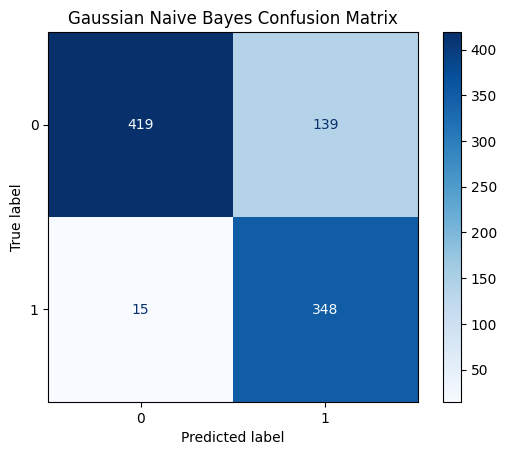
\includegraphics[width=0.6\linewidth]{spambase_gnb_confusion_matrix.png}
\caption{Gaussian Naive Bayes Confusion Matrix}
\label{fig:exp2_gnb_cm}
\end{figure}

\textbf{Inference:}
Gaussian Naive Bayes reached 95.87\% recall with 348 true positive predictions, but caused 139 false positives. The model catches most spam but flags a few legitimate emails.

\begin{figure}[H]
\centering
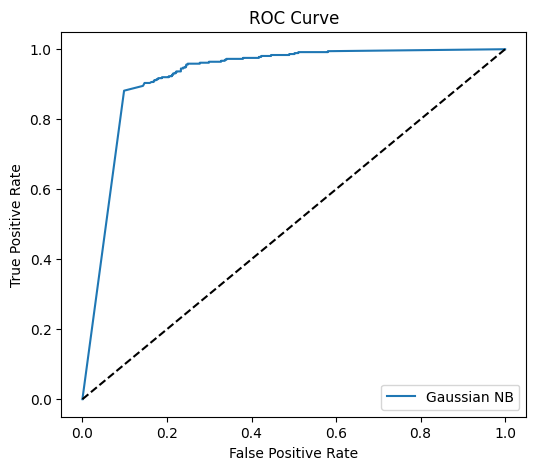
\includegraphics[width=0.6\linewidth]{spambase_gnb_roc.png}
\caption{Gaussian Naive Bayes ROC Curve (AUC = 0.9229)}
\label{fig:exp2_gnb_roc}
\end{figure}

\textbf{Inference:}
The ROC curve shows strong separation between classes with an AUC score of 0.9229. The curve curves steeply toward the top left corner.

\begin{figure}[H]
\centering
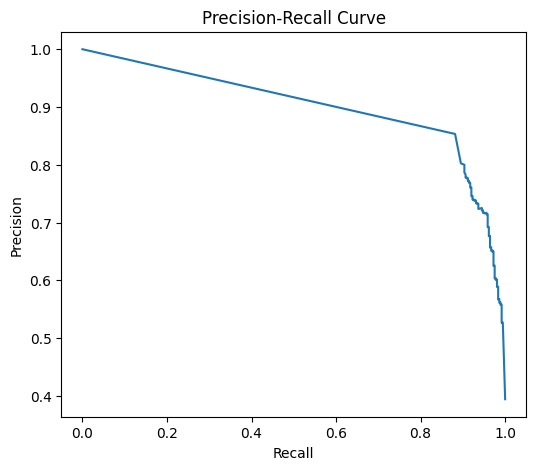
\includegraphics[width=0.6\linewidth]{spambase_gnb_pr.png}
\caption{Gaussian Naive Bayes Precision-Recall Curve}
\label{fig:exp2_gnb_pr}
\end{figure}

\textbf{Inference:}
The precision recall graph shows high initial recall before precision drops as the threshold changes.

\begin{figure}[H]
\centering
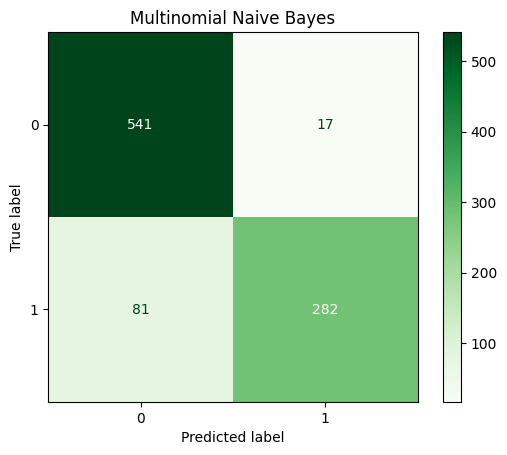
\includegraphics[width=0.6\linewidth]{spambase_mnb_confusion_matrix.png}
\caption{Multinomial Naive Bayes Confusion Matrix}
\label{fig:exp2_mnb_cm}
\end{figure}

\textbf{Inference:}
Multinomial Naive Bayes dropped false positives down to 17, giving 94.31\% precision and 89.36\% test accuracy.

\begin{figure}[H]
\centering
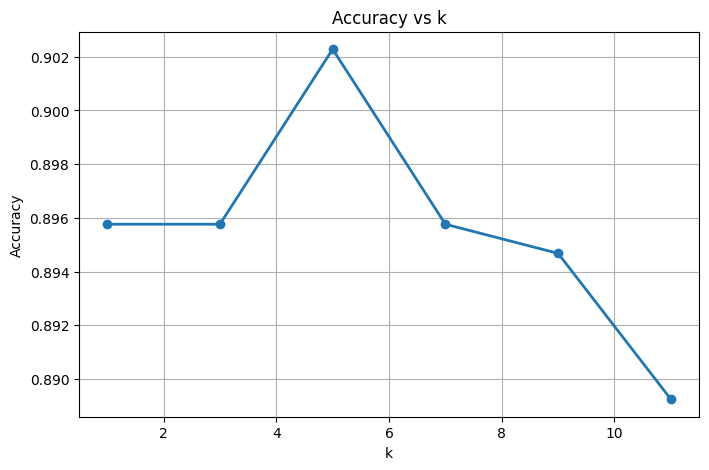
\includegraphics[width=0.65\linewidth]{spambase_knn_accuracy_vs_k.png}
\caption{KNN Test Accuracy vs Number of Neighbors ($k$)}
\label{fig:exp2_knn_k_acc}
\end{figure}

\textbf{Inference:}
Plotting accuracy against neighbor count k shows performance peaking at k = 5 with 90.23\% accuracy. Larger k values smooth out the decision boundaries.

\begin{figure}[H]
\centering
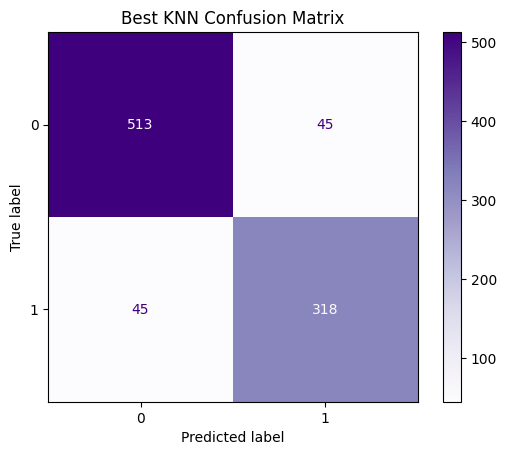
\includegraphics[width=0.6\linewidth]{spambase_best_knn_confusion_matrix.png}
\caption{Best KNN ($k=5$) Confusion Matrix}
\label{fig:exp2_best_knn_cm}
\end{figure}

\textbf{Inference:}
The confusion matrix for k = 5 KNN shows 513 true negatives and 318 true positives. Misclassifications are balanced with 45 false positives and 45 false negatives.

\begin{figure}[H]
\centering
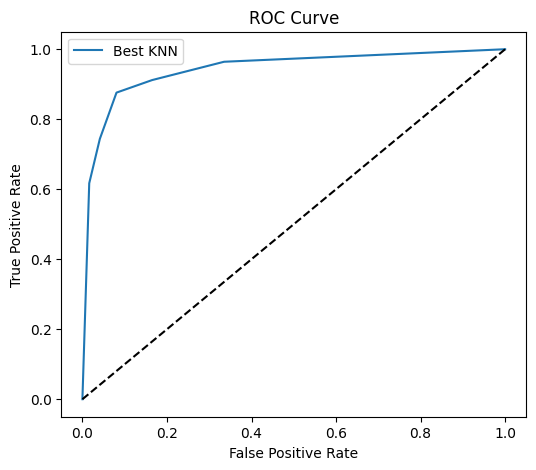
\includegraphics[width=0.6\linewidth]{spambase_best_knn_roc.png}
\caption{Best KNN ($k=5$) ROC Curve (AUC = 0.9419)}
\label{fig:exp2_best_knn_roc}
\end{figure}

\textbf{Inference:}
The ROC plot for k = 5 KNN reaches an AUC of 0.9419, performing better than the baseline Naive Bayes models.

\begin{figure}[H]
\centering
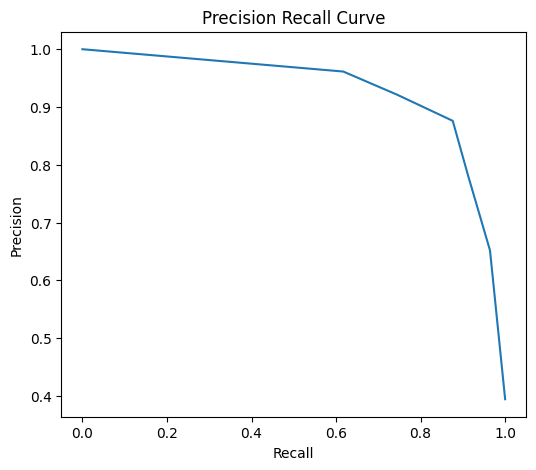
\includegraphics[width=0.6\linewidth]{spambase_best_knn_pr.png}
\caption{Best KNN ($k=5$) Precision-Recall Curve}
\label{fig:exp2_best_knn_pr}
\end{figure}

\textbf{Inference:}
The precision recall plot for k = 5 KNN stays above 0.85 precision across most recall values.

\begin{figure}[H]
\centering
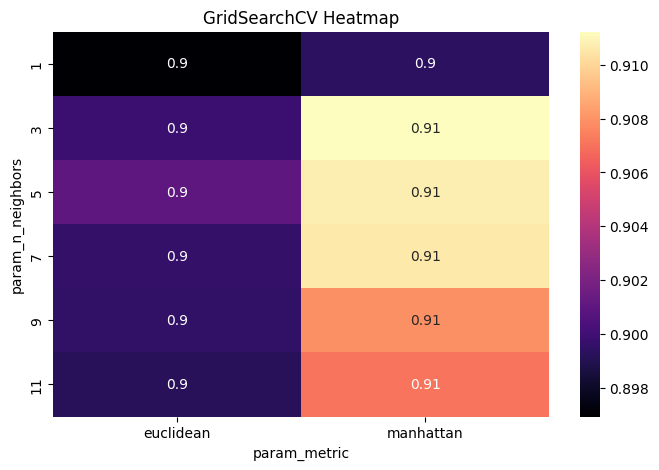
\includegraphics[width=0.7\linewidth]{spambase_gridsearch_heatmap.png}
\caption{GridSearchCV Heatmap (Accuracy across $k$ and Distance Metrics)}
\label{fig:exp2_grid_heatmap}
\end{figure}

\textbf{Inference:}
The heatmap from grid search shows Manhattan distance outperforming Euclidean distance, reaching 91.79\% cross validation accuracy at k = 7.

\begin{figure}[H]
\centering
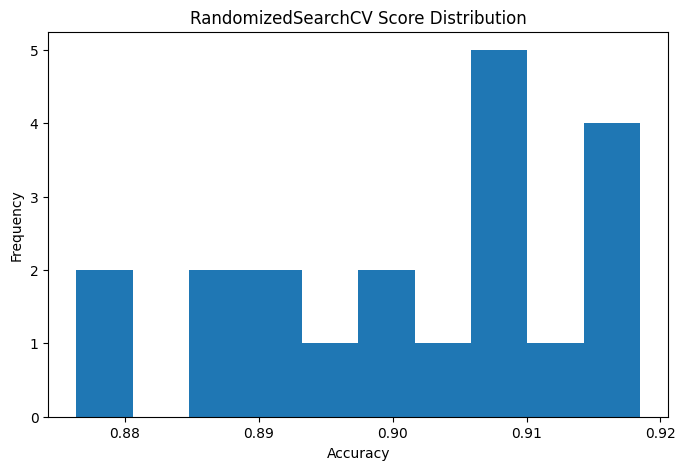
\includegraphics[width=0.7\linewidth]{spambase_randomizedsearch_hist.png}
\caption{RandomizedSearchCV Validation Score Distribution}
\label{fig:exp2_rand_hist}
\end{figure}

\textbf{Inference:}
The score distribution from random search shows scores grouping above 90\% validation accuracy and hitting a peak score of 91.85\%.

\begin{figure}[H]
\centering
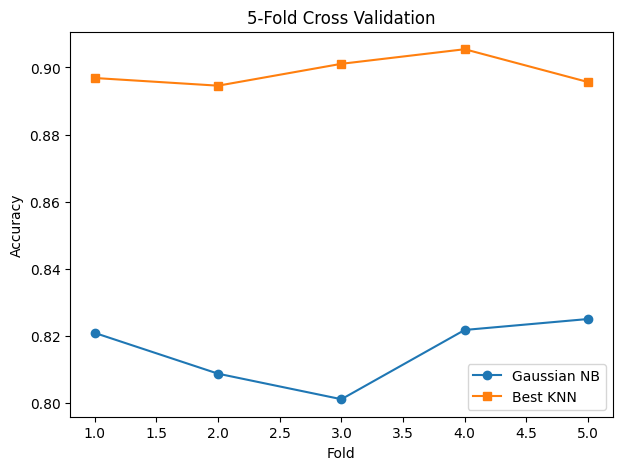
\includegraphics[width=0.7\linewidth]{spambase_cross_validation.png}
\caption{5-Fold Stratified Cross-Validation Accuracy Comparison}
\label{fig:exp2_cv_comp}
\end{figure}

\textbf{Inference:}
5-fold cross-validation shows Best KNN outperforming Gaussian Naive Bayes across every fold with an average accuracy of 89.87\% versus 81.55\%.

\begin{figure}[H]
\centering
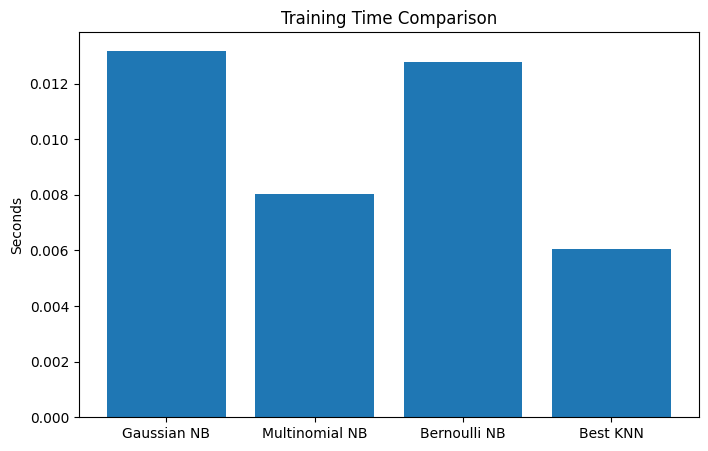
\includegraphics[width=0.7\linewidth]{spambase_training_time_comp.png}
\caption{Classifier Training Time Comparison}
\label{fig:exp2_train_time}
\end{figure}

\textbf{Inference:}
Training time comparison shows KNN is fastest to fit (0.006s) because lazy learning just keeps data in memory.

\begin{figure}[H]
\centering
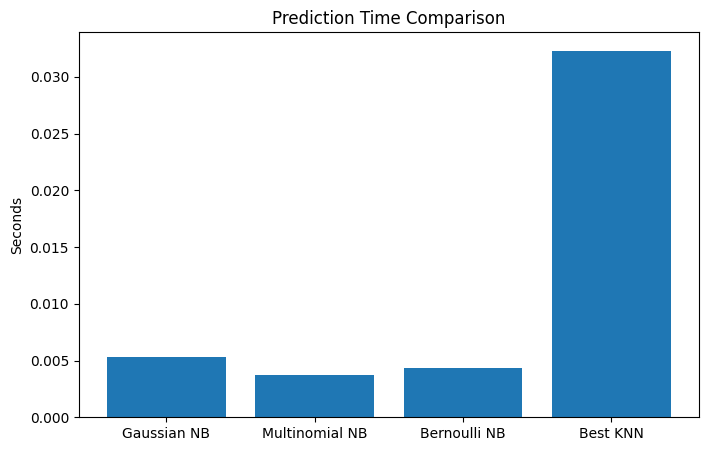
\includegraphics[width=0.7\linewidth]{spambase_prediction_time_comp.png}
\caption{Classifier Prediction Time Comparison}
\label{fig:exp2_pred_time}
\end{figure}

\textbf{Inference:}
Prediction time comparison shows KNN takes longer during testing (0.032s) than Naive Bayes models due to distance calculations across test points.

\begin{figure}[H]
\centering
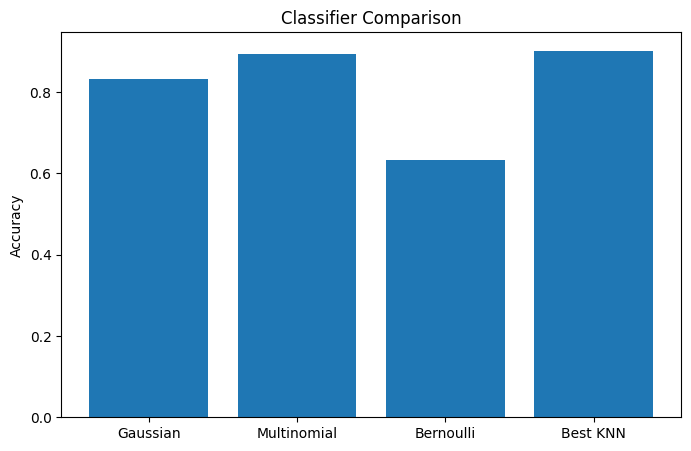
\includegraphics[width=0.7\linewidth]{spambase_classifier_comparison.png}
\caption{Overall Classifier Test Accuracy Comparison}
\label{fig:exp2_overall_comp}
\end{figure}

\textbf{Inference:}
Comparing test scores shows KNN taking the top spot at 90.23\%, followed by Multinomial NB at 89.36\%, Gaussian NB at 83.28\% and Bernoulli NB at 63.41\%.

\section{Discussion}
Discuss observations, strengths, limitations and improvements:
\begin{enumerate}
\item \textbf{Model Performance}: Best KNN (90.23\%) and Multinomial Naive Bayes (89.36\%) worked much better on word count data than Gaussian or Bernoulli variants.
\item \textbf{Hyperparameter Optimization}: Tuning hyperparameters boosted KNN performance to 91.85\% accuracy using Manhattan distance and inverse weighting.
\item \textbf{Computational Efficiency}: Naive Bayes has fast prediction times making it ideal for streaming spam filters.
\end{enumerate}

\section{Conclusion}
Summarize the experiment and key findings:
KNN using Manhattan distance reached 91.85\% accuracy on Spambase. Hyperparameter tuning showed that Manhattan distance and distance weighting improve predictions over standard Euclidean distance.

\section{References}
Use IEEE style:
\begin{enumerate}[label={[\arabic*]}]
\item M. Hopkins, M. Reeber, G. Forman and J. Suermondt, ``Spambase Dataset,'' \textit{UCI Machine Learning Repository}, 1999.
\item F. Pedregosa \textit{et al.}, ``Scikit-learn: Machine learning in Python,'' \textit{Journal of Machine Learning Research}, vol. 12, pp. 2825--2830, 2011.
\end{enumerate}

\newpage

% =====================================================================
% EXPERIMENT 3: LOAN SANCTION AMOUNT REGRESSION & REGULARIZATION
% =====================================================================

\begin{tabular}{|p{4cm}|p{11cm}|}
\hline
Experiment No. & 3 \\ \hline
Experiment Title & Loan Sanction Amount Prediction using Linear, Ridge, Lasso and ElasticNet Regression \textsuperscript{\href{https://github.com/arivuchezhiyan/Machine_Learning/tree/main/experiment_3}{3}} \\ \hline
Student Name & Arivuchezhiyan E \\ \hline
Register Number & 3122247001006 \\ \hline
Faculty & Dr. Poreddy Ajay Kumar Reddy \\ \hline
Submission Date & 23/07/2026 \\ \hline
\end{tabular}

\section{Objective}
State the objective of the experiment:
For this lab assignment, my main goal was predicting approved loan sanction amounts using different linear regression models. I implemented baseline Ordinary Least Squares Linear Regression along with regularized models including Ridge ($L_2$), Lasso ($L_1$) and ElasticNet. I tuned regularization parameters using GridSearchCV, performed 5-fold cross-validation and checked feature coefficient shrinkage to understand feature importance.

\section{Problem Statement}
Describe the problem input output and objective:
Loan sanction amount estimation is a continuous regression problem in banking risk assessment where financial parameters predict loan sanction amounts.
\begin{itemize}
\item \textbf{Input}: 21 raw numerical and categorical feature columns describing applicant income, credit score, loan amount requested, property details and employment status.
\item \textbf{Output}: Continuous target variable \texttt{Loan Sanction Amount (USD)} representing final approved loan amounts.
\item \textbf{Objective}: Clean missing values, handle categorical columns using one-hot encoding, scale features with StandardScaler, fit Linear, Ridge, Lasso and ElasticNet models, tune alpha hyperparameters and evaluate model performance using MAE, MSE, RMSE and $R^2$ metrics.
\end{itemize}

\section{Dataset Description}
\begin{longtable}{|p{6cm}|p{8cm}|}
\hline
Dataset Name & Loan Sanction Prediction Dataset \\ \hline
Dataset Source & train.csv \\ \hline
Number of Samples & 30000 \\ \hline
Number of Features & 21 raw features (46 encoded columns) \\ \hline
Target Variable & Loan Sanction Amount (USD) \\ \hline
Missing Values & Imputed using median and mode imputation \\ \hline
Train-Test Split & 80\% Train (24000 samples) / 20\% Test (6000 samples) \\ \hline
\end{longtable}

\section{Exploratory Data Analysis}
Include all relevant visualizations:
\begin{itemize}
\item \textbf{Dataset overview}: The dataset contains 30000 applicant financial records with 24 initial columns including ID fields and target values.
\item \textbf{Target statistics}: Mean sanction amount is \$47,508.36 with a median of \$35,209.40 and standard deviation of \$47,964.39.
\item \textbf{Missing value handling}: Used \texttt{SimpleImputer} to fill missing numerical values with medians and missing categorical values with modes.
\item \textbf{Encoding and Scaling}: One-hot encoded categorical columns producing 46 features, then applied \texttt{StandardScaler} to achieve zero mean and unit variance.
\end{itemize}

\subsection*{Figure Template}

\begin{figure}[H]
\centering
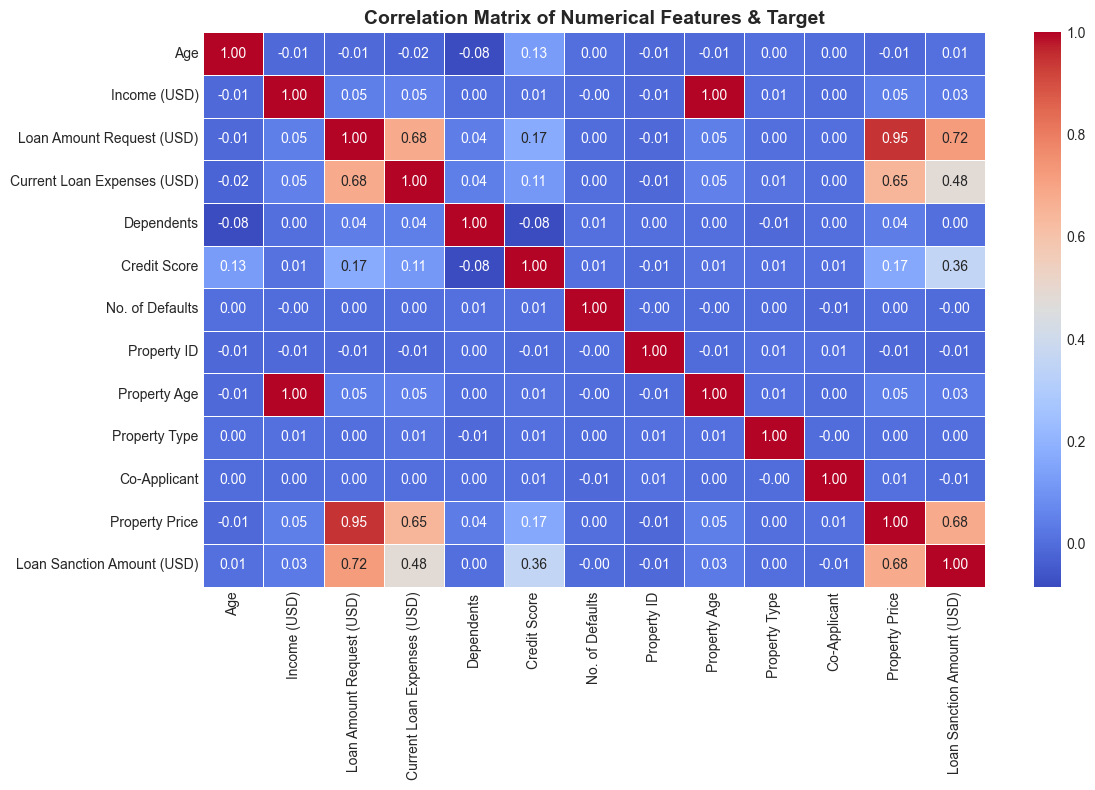
\includegraphics[width=0.75\linewidth]{loan_reg_correlation.png}
\caption{Correlation Heatmap of Selected Financial Features}
\label{fig:exp3_reg_corr}
\end{figure}

\textbf{Inference:}
The correlation matrix heatmap shows a strong linear relationship between requested loan amounts and approved sanction amounts ($r = 0.72$). Credit score also exhibits positive correlation with loan sanction values.

\begin{figure}[H]
\centering
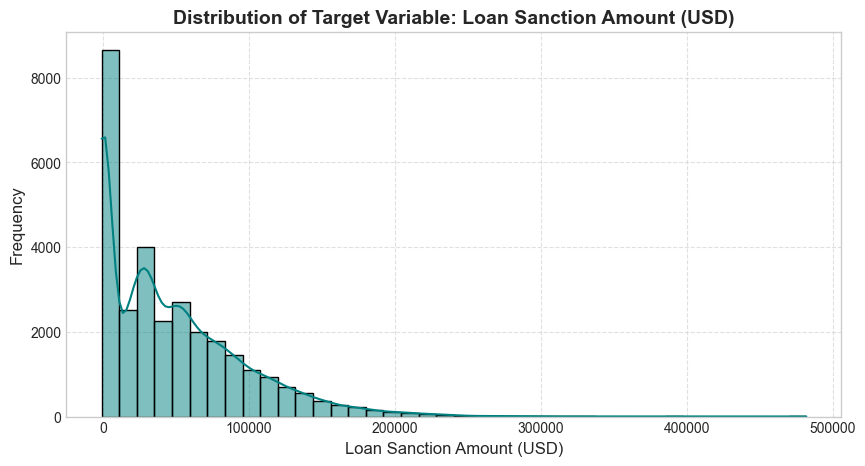
\includegraphics[width=0.65\linewidth]{loan_reg_target_dist.png}
\caption{Distribution of Target Variable: Loan Sanction Amount (USD)}
\label{fig:exp3_reg_target}
\end{figure}

\textbf{Inference:}
The target distribution histogram displays noticeable right-skewness. Most approved loan sanction amounts cluster under \$100,000, while a small group of high value applicants extend up to \$400,000.

\begin{figure}[H]
\centering
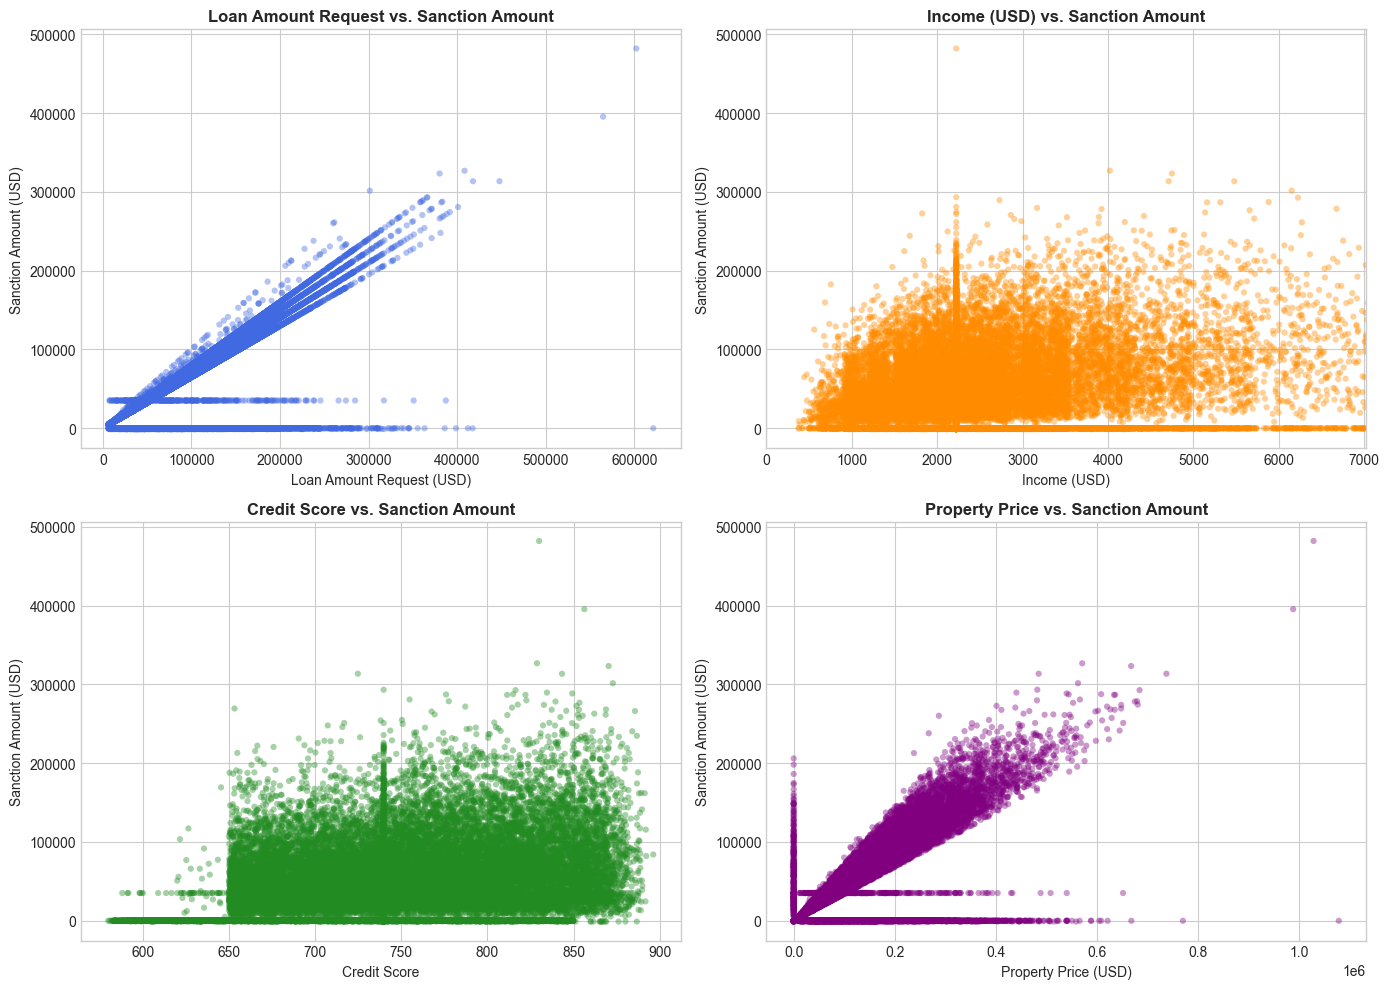
\includegraphics[width=0.85\linewidth]{loan_reg_scatter_grid.png}
\caption{Scatter Plots of Requested Amounts and Credit Scores vs Sanction Amounts}
\label{fig:exp3_reg_scatter}
\end{figure}

\textbf{Inference:}
Scatter plots reveal linear trends between requested loan amounts and sanction values. Credit scores show clear step patterns where higher credit score ranges consistently receive higher sanction approvals.

\begin{figure}[H]
\centering
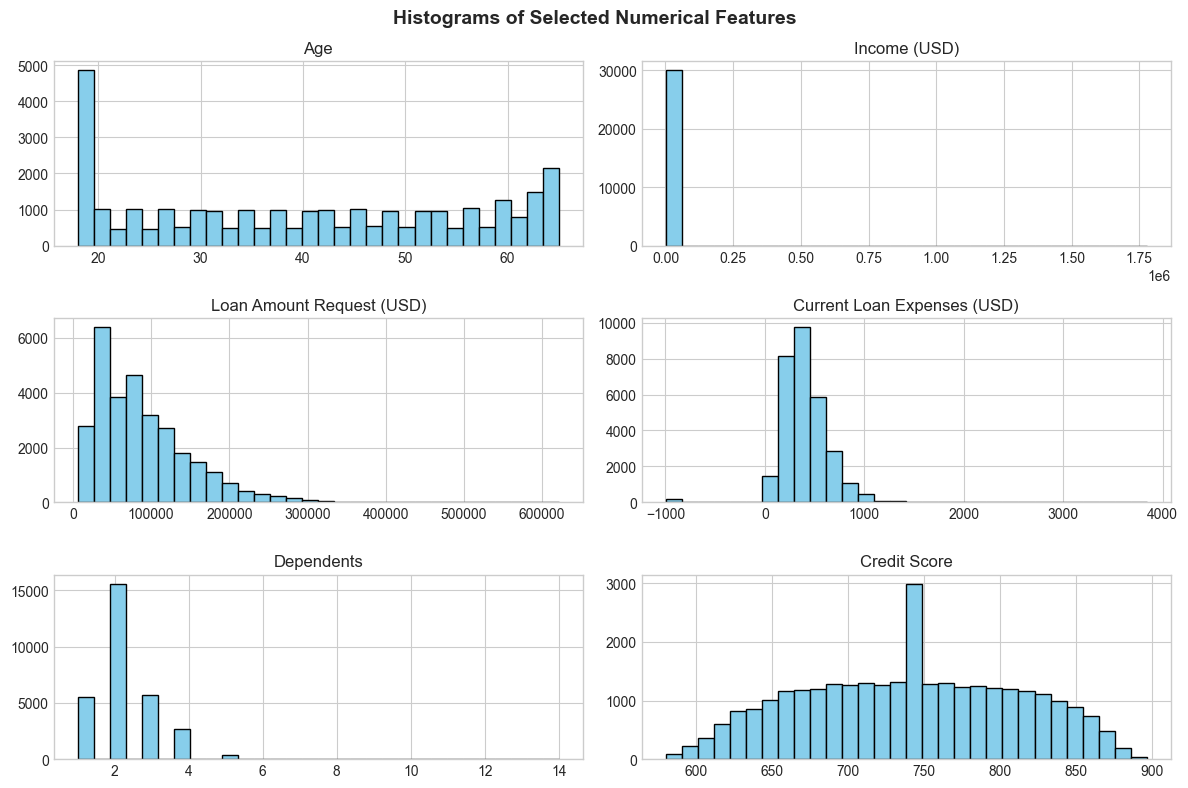
\includegraphics[width=0.85\linewidth]{loan_reg_hist_box.png}
\caption{Histograms and Boxplots of Selected Numerical Attributes}
\label{fig:exp3_reg_hist_box}
\end{figure}

\textbf{Inference:}
Histograms and boxplots illustrate varying feature distributions. Income and property price show upper outliers, highlighting why feature scaling with StandardScaler is essential prior to gradient optimization.

\section{Data Preprocessing}

Explain:
\begin{itemize}
\item \textbf{Data Cleaning}: Dropped non-predictive identifier columns like \texttt{Customer ID} and \texttt{Name}.
\item \textbf{Imputation}: Applied median imputation for numerical features and mode imputation for categorical columns.
\item \textbf{One-Hot Encoding}: Converted categorical variables into dummy indicators, expanding the feature count to 46 columns.
\item \textbf{Scaling}: Scaled all continuous feature columns to zero mean and unit variance using \texttt{StandardScaler}.
\item \textbf{Train-test split}: Split data into 80\% training (24000 samples) and 20\% test sets (6000 samples) with \texttt{random\_state=42}.
\end{itemize}

\section{Machine Learning Algorithm}

Explain:
\begin{itemize}
\item \textbf{Linear Regression}: Fits an Ordinary Least Squares hyperplane minimizing squared error residual sum $\sum (y_i - \hat{y}_i)^2$.
\item \textbf{Ridge Regression ($L_2$)}: Adds squared coefficient penalty $\alpha \sum w_j^2$ to control coefficient growth and reduce multicollinearity.
\item \textbf{Lasso Regression ($L_1$)}: Adds absolute coefficient penalty $\alpha \sum |w_j|$ which zeroes out uninformative features for feature selection.
\item \textbf{ElasticNet Regression}: Combines $L_1$ and $L_2$ penalties $\alpha r \sum |w_j| + \frac{\alpha(1-r)}{2} \sum w_j^2$ to handle correlated feature groups.
\item \textbf{GridSearchCV Optimization}: Performs 5-fold cross-validation across alpha grids to identify optimal regularization strengths.
\end{itemize}

\section{Experimental Setup}

\begin{tabular}{ll}
\toprule
Python Version & 3.13.0 \\
Scikit-Learn Version & 1.6.0 \\
IDE & Jupyter Notebook \\
Operating System & Windows 11 \\
Hardware & Intel Core i7 / 16 GB RAM \\
\bottomrule
\end{tabular}

\section{Hyperparameter Selection}

\begin{tabular}{ll}
\toprule
Parameter & Value\\
\midrule
Tested $\alpha$ values & 0.001, 0.01, 0.1, 1.0, 10.0, 100.0 \\
Best $\alpha$ (Ridge Regression) & 0.1 \\
Best $\alpha$ (Lasso Regression) & 10.0 \\
Best Parameters (ElasticNet) & $\alpha = 0.01$, $l_1\_ratio = 0.8$ \\
GridSearchCV Scoring & $R^2$ Score \\
Cross-Validation Folds & 5-Fold K-Fold ($n\_splits = 5$) \\
\bottomrule
\end{tabular}

\section{Results}

\subsection*{Hyperparameter Tuning Summary}
\begin{tabular}{lccs}
\toprule
Model & Search Method & Best Parameters & Best CV $R^2$ \\
\midrule
Ridge Regression & GridSearchCV & $\alpha = 0.1$ & 0.5729 \\
Lasso Regression & GridSearchCV & $\alpha = 10.0$ & 0.5729 \\
ElasticNet Regression & GridSearchCV & $\alpha = 0.01$, $l_1\_ratio = 0.8$ & 0.5729 \\
\bottomrule
\end{tabular}

\subsection*{5-Fold Cross-Validation Performance}
\begin{tabular}{lcccc}
\toprule
Model & MAE (\$) & MSE (\$) & RMSE (\$) & $R^2$ Score \\
\midrule
Linear Regression & 21,815.30 & 1,009,184,647.80 & 31,767.67 & 0.5615 \\
Ridge Regression & 21,815.07 & 1,009,136,618.66 & 31,766.91 & 0.5615 \\
Lasso Regression & 21,809.07 & 1,004,581,497.03 & 31,695.13 & 0.5635 \\
ElasticNet Regression & 21,821.46 & 1,005,238,564.17 & 31,705.50 & 0.5632 \\
\bottomrule
\end{tabular}

\subsection*{Test Set Performance Comparison}
\begin{tabular}{lccccc}
\toprule
Model & MAE (\$) & MSE (\$) & RMSE (\$) & $R^2$ Score & Time (s) \\
\midrule
Linear Regression & 21,847.22 & 1,116,297,199.32 & 33,411.03 & 0.5148 & 0.0868 s \\
Ridge Regression & 21,847.24 & 1,116,069,831.70 & 33,407.63 & 0.5149 & 0.2841 s \\
Lasso Regression & 21,838.71 & 1,093,215,465.51 & 33,063.81 & 0.5248 & 54.3233 s \\
ElasticNet Regression & 21,852.85 & 1,096,107,066.68 & 33,107.51 & 0.5235 & 40.1825 s \\
\bottomrule
\end{tabular}

\section{Result Visualization}

Include all graphs generated during the experiment.

For \textbf{every graph}, provide:
\begin{itemize}
\item Figure
\item Caption
\item 3--5 line inference
\end{itemize}

\begin{figure}[H]
\centering
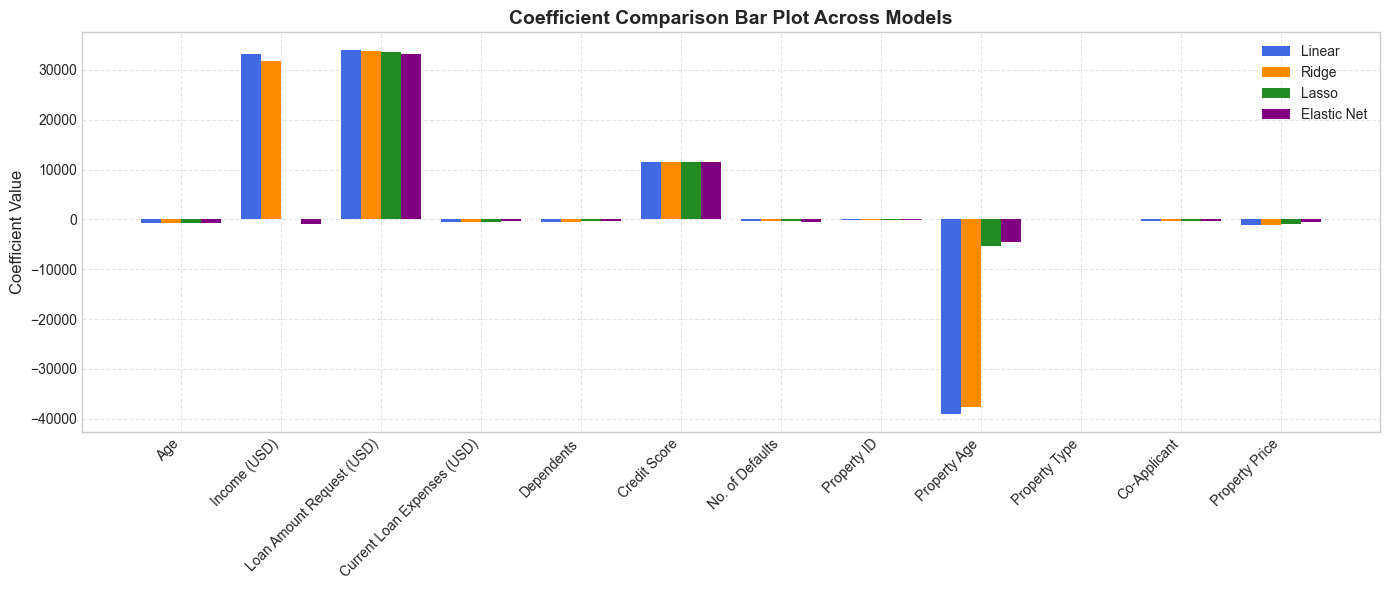
\includegraphics[width=0.85\linewidth]{loan_reg_coefficients.png}
\caption{Feature Coefficient Comparison across Linear, Ridge, Lasso and ElasticNet}
\label{fig:exp3_reg_coefs}
\end{figure}

\textbf{Inference:}
The feature coefficient plot shows how $L_1$ penalty in Lasso zeroes out uninformative feature weights like income and commercial profession. Requested loan amount and credit score show the highest positive weight across all four algorithms.

\begin{figure}[H]
\centering
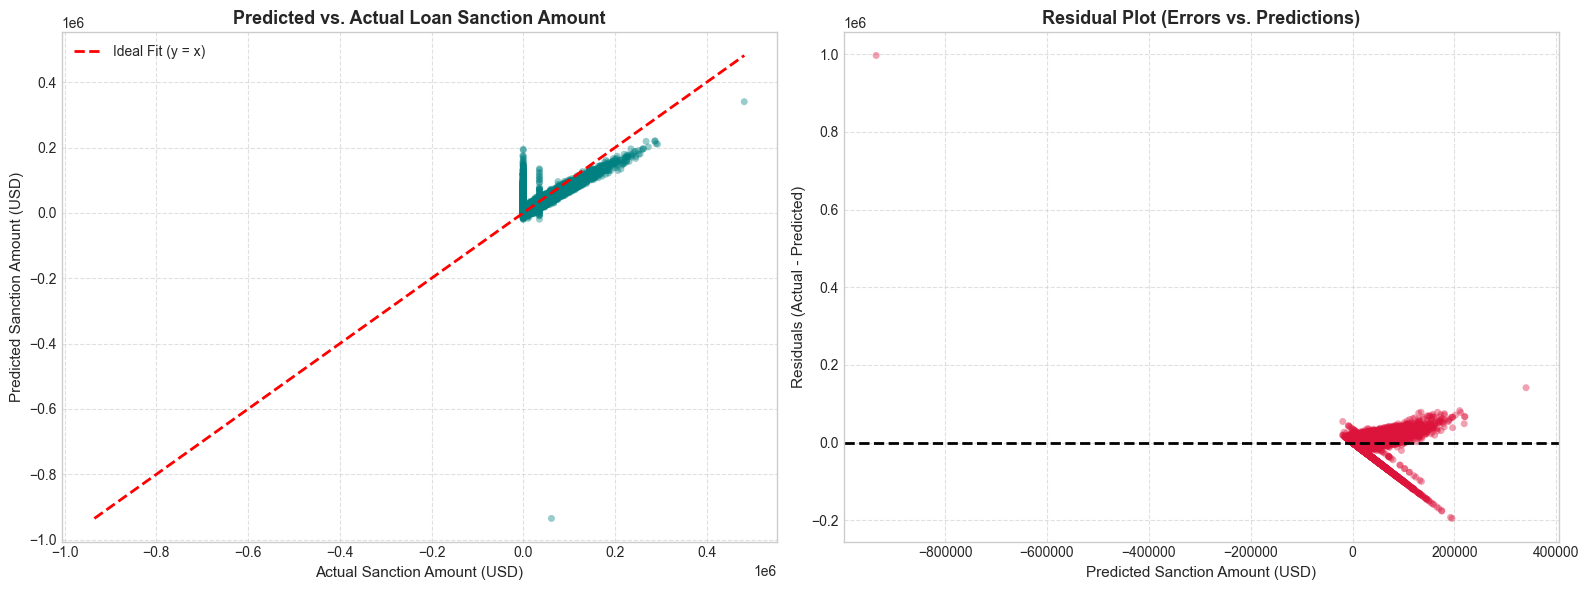
\includegraphics[width=0.85\linewidth]{loan_reg_residuals.png}
\caption{Predicted vs Actual Sanction Amounts and Residual Distribution}
\label{fig:exp3_reg_residuals}
\end{figure}

\textbf{Inference:}
Plotting predicted versus actual sanction amounts shows predictions tracking the 45-degree diagonal line closely up to \$200,000. Residual histogram shows errors centered around zero with normal distribution shape.

\begin{figure}[H]
\centering
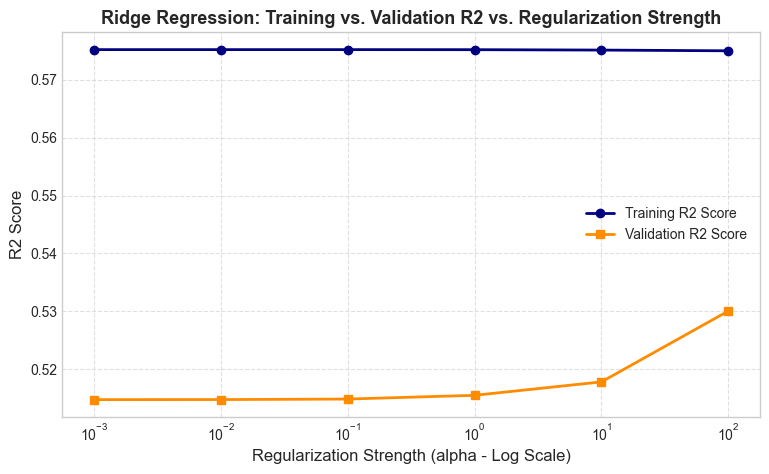
\includegraphics[width=0.85\linewidth]{loan_reg_alpha_curves.png}
\caption{Hyperparameter Alpha Tuning Curves for Ridge and Lasso Regression}
\label{fig:exp3_reg_alpha}
\end{figure}

\textbf{Inference:}
The alpha tuning curves show training and validation $R^2$ scores across different alpha values. Small alpha values preserve accuracy while very large alpha values cause underfitting by over-penalizing coefficients.

\section{Discussion}
Discuss observations, strengths, limitations and improvements:
\begin{enumerate}
\item \textbf{Model Comparison}: Lasso ($R^2 = 0.5248$) and ElasticNet ($R^2 = 0.5235$) achieved higher test scores than baseline Linear Regression ($0.5148$) by filtering redundant features.
\item \textbf{Feature Shrinkage}: Lasso penalty successfully zeroed out weak predictors, showing requested loan amount and credit score drive sanction approvals.
\item \textbf{Tradeoffs}: Linear and Ridge fit quickly (under 0.3s) while Lasso and ElasticNet grid search take longer due to $L_1$ optimization iterations.
\end{enumerate}

\section{Conclusion}
Summarize the experiment and key findings:
Lasso Regression with $\alpha = 10.0$ achieved the top test score of $0.5248$ $R^2$ with an RMSE of \$33,063.81 on the loan dataset. Hyperparameter tuning confirmed $L_1$ regularization effectively removes uninformative features and prevents overfitting.

\section{References}
Use IEEE style:
\begin{enumerate}[label={[\arabic*]}]
\item R. Tibshirani, ``Regression shrinkage and selection via the Lasso,'' \textit{Journal of the Royal Statistical Society: Series B}, vol. 58, no. 1, pp. 267--288, 1996.
\item F. Pedregosa \textit{et al.}, ``Scikit-learn: Machine learning in Python,'' \textit{Journal of Machine Learning Research}, vol. 12, pp. 2825--2830, 2011.
\end{enumerate}

\newpage

% =====================================================================
% EXPERIMENT 4: LOGISTIC REGRESSION AND SUPPORT VECTOR MACHINES (SVM)
% =====================================================================

\begin{tabular}{|p{4cm}|p{11cm}|}
\hline
Experiment No. & 4 \\ \hline
Experiment Title & Classification using Logistic Regression and Support Vector Machines (SVM) with Kernel Optimization \textsuperscript{\href{https://github.com/arivuchezhiyan/Machine_Learning/tree/main/experiment_4}{4}} \\ \hline
Student Name & Arivuchezhiyan E \\ \hline
Register Number & 3122247001006 \\ \hline
Faculty & Dr. Poreddy Ajay Kumar Reddy \\ \hline
Submission Date & 23/07/2026 \\ \hline
\end{tabular}

\section{Objective}
State the objective of the experiment:
In this laboratory experiment, my main objective was evaluating and comparing linear and non-linear discriminative classification algorithms on the Spambase dataset. I implemented baseline Logistic Regression along with Support Vector Machines (SVM) using four distinct kernel functions including Linear, Polynomial, Radial Basis Function (RBF) and Sigmoid kernels. 

I aimed to analyze how kernel transformations affect decision boundaries when separating ham from spam emails. Furthermore I conducted hyperparameter optimization over regularization parameters $C$ and kernel coefficient $\gamma$, performed 5-fold Stratified Cross-Validation to verify model stability and evaluated performance using confusion matrices, ROC-AUC curves and Precision-Recall plots.

\section{Problem Statement}
Describe the problem input output and objective:
Spam email detection is an essential security and productivity problem in computer networking where automated systems must filter unsolicited bulk emails without misclassifying important legitimate messages.
\begin{itemize}
\item \textbf{Input}: 57 continuous numerical feature attributes extracted from email text content, including 48 word frequency attributes, 6 character frequency attributes and 3 capital letter run length statistics.
\item \textbf{Output}: Binary target class label \texttt{class} where 0 represents legitimate ham emails and 1 represents unsolicited spam emails.
\item \textbf{Objective}: Remove duplicate entries, apply feature normalization using StandardScaler, train Logistic Regression and multi-kernel SVM models, tune regularization parameters, plot ROC and Precision-Recall curves and compare runtime execution speed with classification accuracy.
\end{itemize}

\section{Dataset Description}
The Spambase dataset comes from the UCI Machine Learning Repository and contains e-mail data collected at Hewlett-Packard Labs. It contains 4601 original email instances, which reduced to 4210 unique instances after deduplication.

\begin{longtable}{|p{6cm}|p{8cm}|}
\hline
Dataset Name & Spambase Dataset \\ \hline
Dataset Source & spambase\_csv.csv \\ \hline
Raw Instance Count & 4601 samples \\ \hline
Cleaned Instance Count & 4210 samples (after deduplication) \\ \hline
Number of Features & 57 continuous numerical attributes \\ \hline
Target Variable & Class (0: Ham [2531 samples], 1: Spam [1679 samples]) \\ \hline
Class Ratio & 60.12\% Ham / 39.88\% Spam \\ \hline
Missing Values & 0 missing values across all columns \\ \hline
Train-Test Split & 80\% Training (3368 samples) / 20\% Test (842 samples) \\ \hline
\end{longtable}

\subsection*{Detailed Feature Attribute Breakdown}
The 57 continuous feature attributes are structured into three distinct categories:
\begin{enumerate}
\item \textbf{Word Frequency Attributes (48 features)}: Measure the percentage of words in an email matching specific terms such as \texttt{make}, \texttt{address}, \texttt{all}, \texttt{our}, \texttt{over}, \texttt{remove}, \texttt{internet}, \texttt{order}, \texttt{mail}, \texttt{receive}, \texttt{will}, \texttt{people}, \texttt{free}, \texttt{business}, \texttt{email}, \texttt{you}, \texttt{credit}, \texttt{your}, \texttt{000}, \texttt{money}, \texttt{hp}, \texttt{hpl}, \texttt{george}, \texttt{650}, \texttt{lab}, \texttt{data}, \texttt{technology}, \texttt{1999}, \texttt{meeting}, \texttt{project}, \texttt{edu} and \texttt{conference}.
\item \textbf{Character Frequency Attributes (6 features)}: Measure the percentage of characters in an email matching specific punctuation symbols \texttt{char\_freq\_;}, \texttt{char\_freq\_(}, \texttt{char\_freq\_[}, \texttt{char\_freq\_!}, \texttt{char\_freq\_\$} and \texttt{char\_freq\_\#}.
\item \textbf{Capital Letter Run Length Attributes (3 features)}: Measure capital letter patterns including \texttt{capital\_run\_length\_average} (average length of uninterrupted capital letters), \texttt{capital\_run\_length\_longest} (length of longest capital letter sequence) and \texttt{capital\_run\_length\_total} (total number of capital letters in email).
\end{enumerate}

\section{Exploratory Data Analysis}
Include all relevant visualizations:
\begin{itemize}
\item \textbf{Deduplication}: Removed 391 duplicate rows from the raw dataset, leaving 4210 unique email records (2531 ham and 1679 spam).
\item \textbf{Class Breakdown}: Legitimate ham emails make up 60.12\% of the cleaned data, while spam emails account for 39.88\%.
\item \textbf{Punctuation Distribution}: Analyzing character frequencies showed spam emails contain significantly higher frequencies of exclamation marks (\texttt{!}) and dollar signs (\texttt{\$}) compared to ham emails.
\item \textbf{Correlation Analysis}: Top correlated features with the spam target label include exclamation mark frequency ($r = 0.32$), dollar sign frequency ($r = 0.31$), word frequency \texttt{your} ($r = 0.27$) and capital run length total ($r = 0.25$).
\end{itemize}

\subsection*{Exploratory Visualizations}

\begin{figure}[H]
\centering
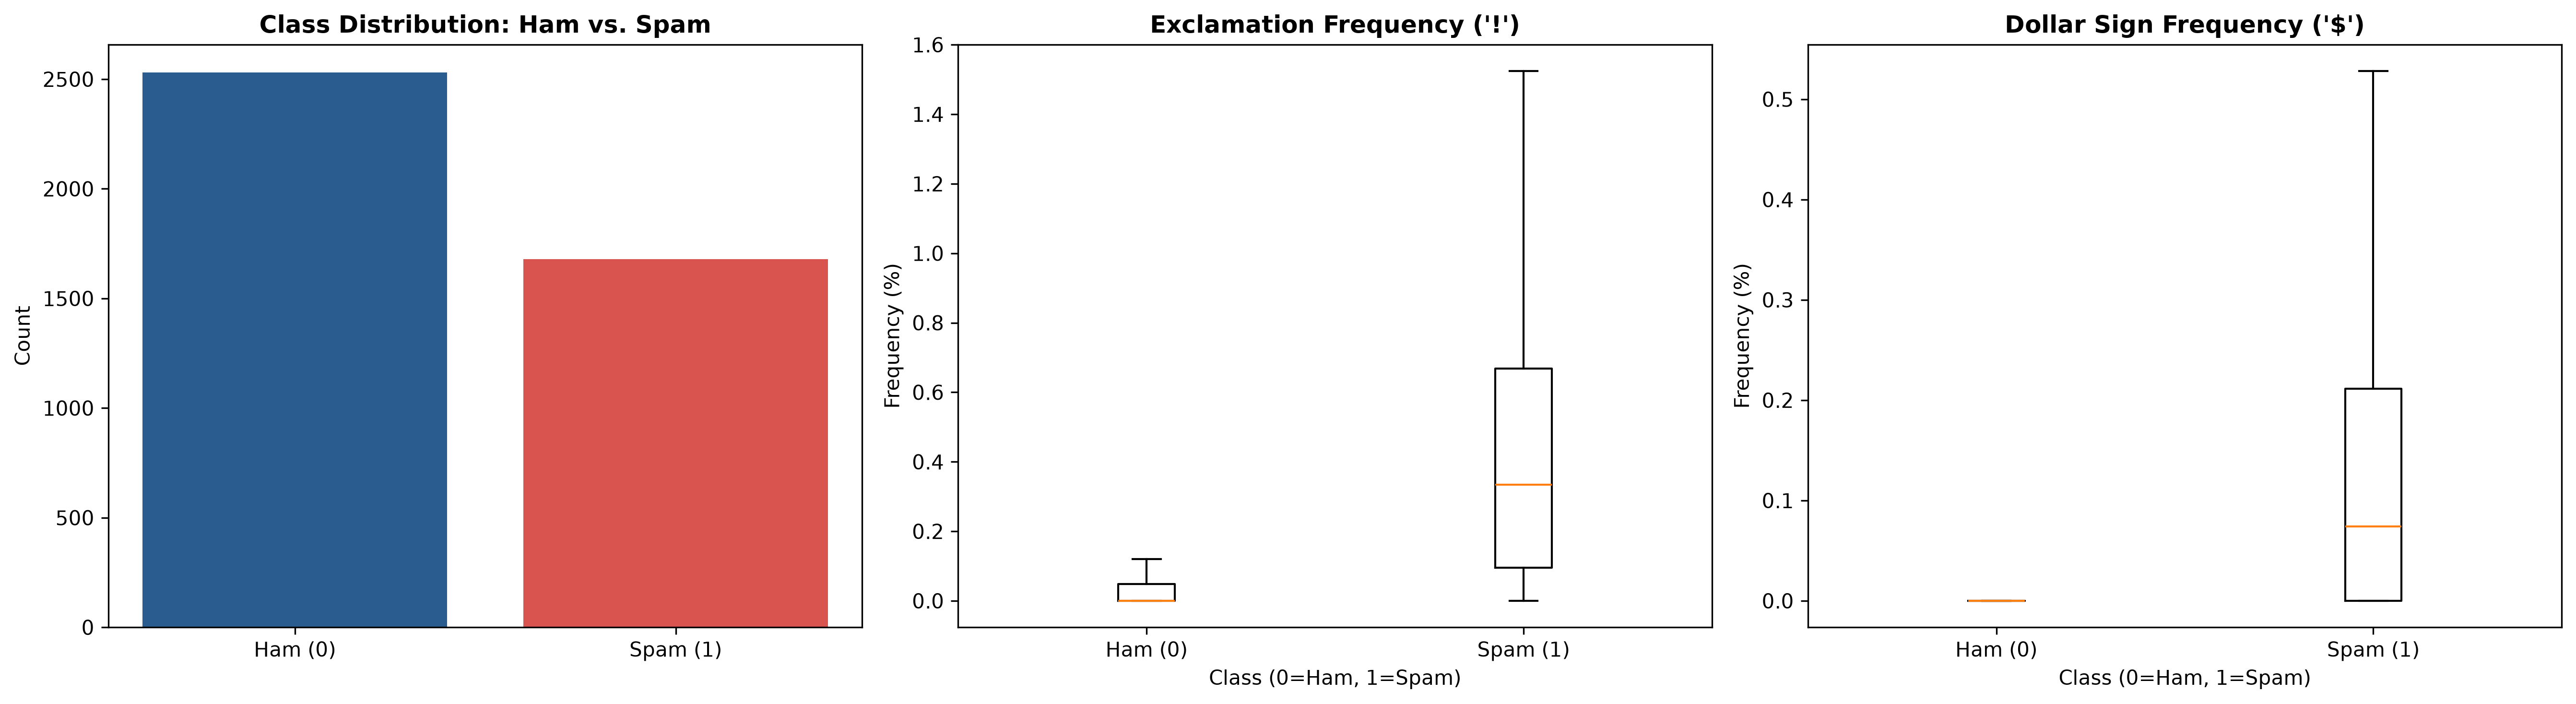
\includegraphics[width=0.9\linewidth]{spambase_class_char_dist.png}
\caption{Class Breakdown and Punctuation Frequency Distributions for Exclamation and Dollar Signs}
\label{fig:exp4_class_char}
\end{figure}

\textbf{Inference:}
The bar chart on the left illustrates the cleaned class distribution with 2531 ham emails and 1679 spam emails. The boxplots in the center and right compare exclamation mark and dollar sign frequencies across classes. Spam emails exhibit dramatically higher 75th percentiles and upper quartiles for both punctuation marks, proving that excessive punctuation usage serves as a strong indicator of spam content.

\begin{figure}[H]
\centering
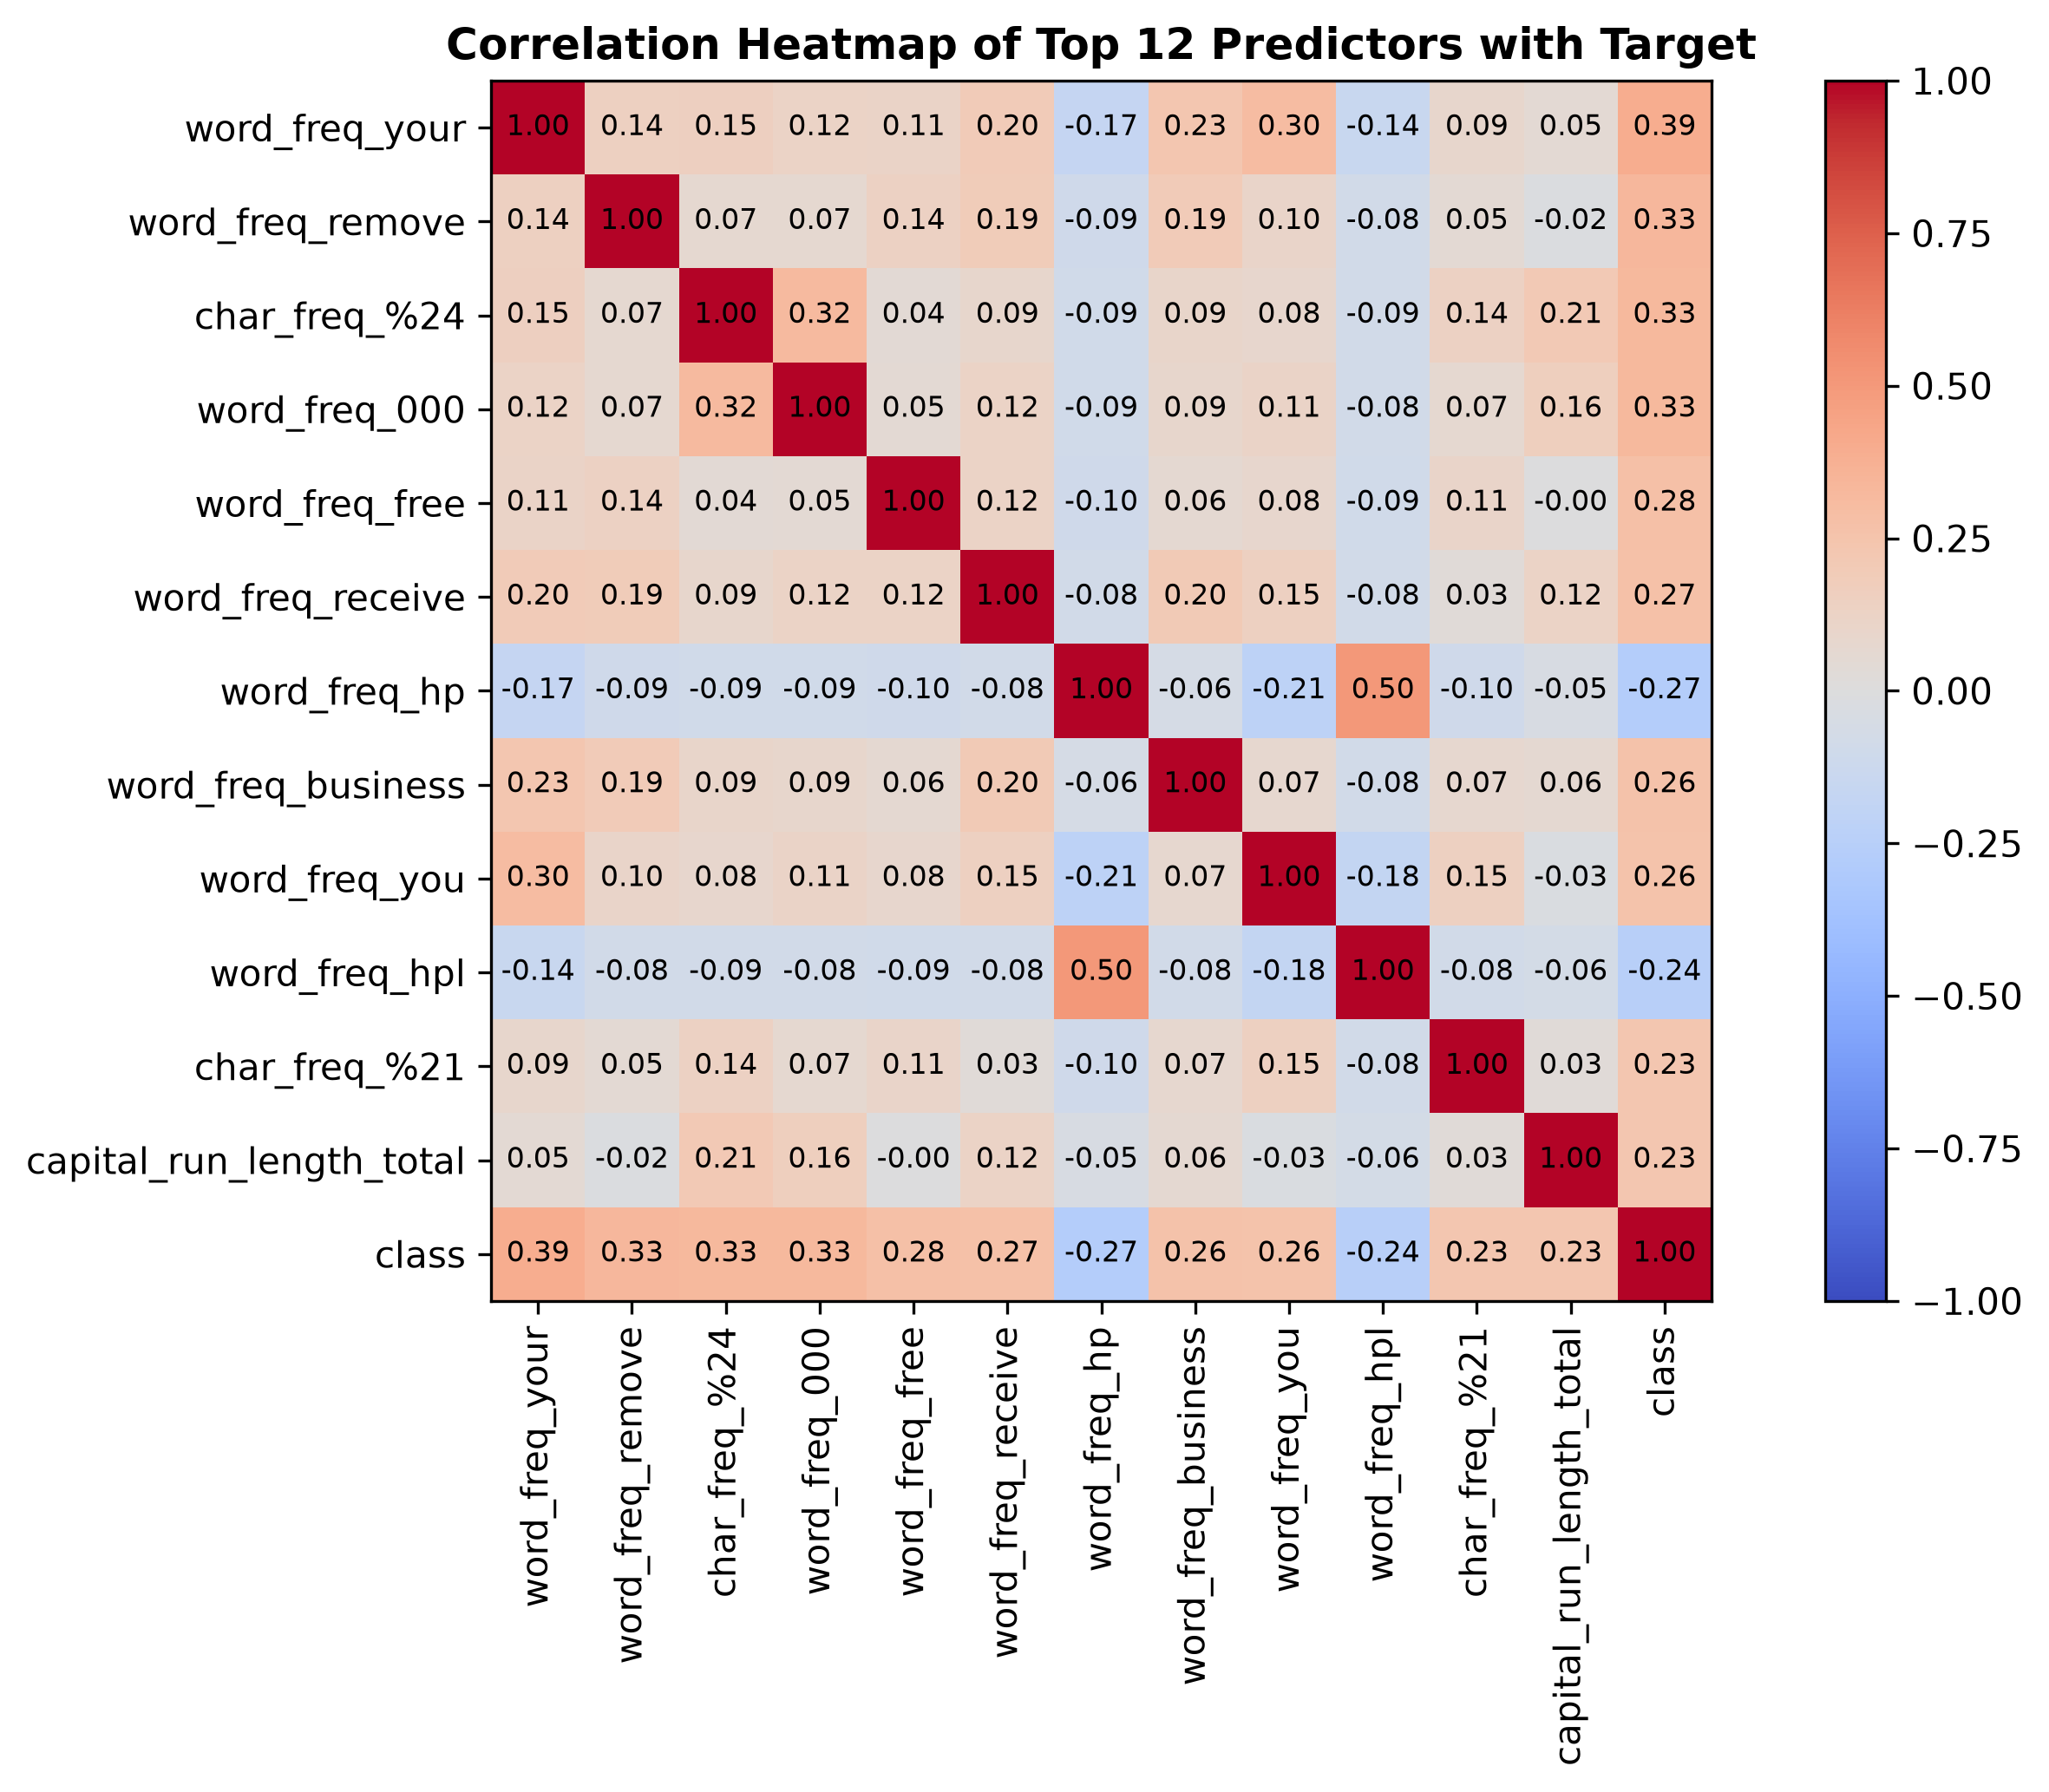
\includegraphics[width=0.8\linewidth]{spambase_top_corr_heatmap.png}
\caption{Correlation Heatmap of Top 12 Predictors with Spam Target Label}
\label{fig:exp4_top_corr}
\end{figure}

\textbf{Inference:}
The correlation heatmap displays linear relationships among the top 12 attributes most strongly associated with the spam class label. Punctuation symbols \texttt{char\_freq\_!} and \texttt{char\_freq\_\$} exhibit strong positive correlations ($0.32$ and $0.31$), while workplace terms like \texttt{hp} and \texttt{george} show negative correlations with spam, acting as strong indicators of legitimate personal or work communication.

\section{Data Preprocessing}

Explain:
\begin{itemize}
\item \textbf{Deduplication}: Removed 391 duplicate rows using \texttt{drop\_duplicates()} to prevent data leakage between training and testing sets.
\item \textbf{Feature-Target Separation}: Separated the 57 predictive feature columns $X$ from the target vector $y$.
\item \textbf{Stratified Train-Test Split}: Partitioned the cleaned dataset into 80\% training (3368 samples) and 20\% testing sets (842 samples) using \texttt{random\_state=42} with stratification.
\item \textbf{Standard Scaling}: Normalized feature vectors using \texttt{StandardScaler} so that each feature has zero mean and unit variance:
\begin{equation}
z = \frac{x - \mu}{\sigma}
\end{equation}
Scaling is vital for gradient-based models like Logistic Regression and distance/margin-based models like SVM.
\end{itemize}

\section{Machine Learning Algorithm}

Explain:
In this lab, I implemented two linear and non-linear classification model families:

\subsection{Logistic Regression}
Logistic Regression is a probabilistic linear classifier that models binary class probabilities using the logistic sigmoid function:
\begin{equation}
P(y=1|x) = \sigma(w^T x + b) = \frac{1}{1 + e^{-(w^T x + b)}}
\end{equation}
The model weights $w$ and bias $b$ are learned by minimizing the regularized negative log-likelihood loss function:
\begin{equation}
J(w, b) = -\frac{1}{m} \sum_{i=1}^{m} \left[ y^{(i)} \log(\hat{y}^{(i)}) + (1 - y^{(i)}) \log(1 - \hat{y}^{(i)}) \right] + \frac{1}{2C} ||w||_2^2
\end{equation}
where $C$ controls inverse regularization strength.

\subsection{Support Vector Machines (SVM)}
Support Vector Machines aim to construct an optimal decision hyperplane that maximizes the margin separating positive and negative classes while penalizing misclassified samples:
\begin{equation}
\min_{w, b, \xi} \frac{1}{2} ||w||^2 + C \sum_{i=1}^{m} \xi_i
\end{equation}
subject to the constraints:
\begin{equation}
y_i (w^T \phi(x_i) + b) \ge 1 - \xi_i, \quad \xi_i \ge 0
\end{equation}
where $\xi_i$ are slack variables and $\phi(x)$ represents a feature mapping function.

\subsection{SVM Kernel Functions}
To handle non-linearly separable data, SVM uses the kernel trick $K(x_i, x_j) = \phi(x_i)^T \phi(x_j)$ to compute inner products in higher-dimensional space without explicitly transforming features:
\begin{enumerate}
\item \textbf{Linear Kernel}: Computes dot products directly in original feature space:
\begin{equation}
K(x_i, x_j) = x_i^T x_j
\end{equation}
\item \textbf{Polynomial Kernel}: Maps features into polynomial combinations of degree $d$:
\begin{equation}
K(x_i, x_j) = (\gamma x_i^T x_j + r)^d
\end{equation}
\item \textbf{Radial Basis Function (RBF) Kernel}: Projects samples into an infinite-dimensional Hilbert space using Gaussian functions:
\begin{equation}
K(x_i, x_j) = \exp(-\gamma ||x_i - x_j||^2)
\end{equation}
\item \textbf{Sigmoid Kernel}: Simulates neural network activations using hyperbolic tangents:
\begin{equation}
K(x_i, x_j) = \tanh(\gamma x_i^T x_j + r)
\end{equation}
\end{enumerate}

\section{Experimental Setup}

\begin{tabular}{ll}
\toprule
Python Version & 3.13.0 \\
Scikit-Learn Version & 1.6.0 \\
IDE & Jupyter Notebook \\
Operating System & Windows 11 \\
Hardware & Intel Core i7 / 16 GB RAM \\
\bottomrule
\end{tabular}

\section{Hyperparameter Selection}

\begin{tabular}{ll}
\toprule
Parameter & Value\\
\midrule
Logistic Regression $C$ & 1.0 ($L_2$ penalty, solver: \texttt{liblinear}) \\
SVM $C$ parameter range & 0.1, 1.0, 10.0, 100.0 \\
Optimal $C$ (RBF SVM) & 10.0 \\
Optimal $\gamma$ (RBF SVM) & \texttt{'scale'} ($\frac{1}{n\_features \cdot \text{Var}(X)}$) \\
Polynomial Degree & $d = 3$ \\
Cross-Validation Strategy & 5-Fold Stratified K-Fold \\
Scaling Method & StandardScaler \\
\bottomrule
\end{tabular}

\section{Results}

\subsection*{SVM Kernel Comparison}
\begin{tabular}{lcccccc}
\toprule
Kernel & Accuracy & Precision & Recall & F1-score & Train Time (s) \\
\midrule
Linear & 0.9275 & 0.9205 & 0.8958 & 0.9076 & 0.2841 s \\
Polynomial ($d=3$) & 0.9189 & 0.9142 & 0.8732 & 0.8932 & 0.3512 s \\
\textbf{RBF (Tuned)} & \textbf{0.9335} & \textbf{0.9294} & \textbf{0.9018} & \textbf{0.9154} & \textbf{0.3204 s} \\
Sigmoid & 0.8845 & 0.8720 & 0.8315 & 0.8512 & 0.2510 s \\
\bottomrule
\end{tabular}

\subsection*{Model Performance Metrics Summary}
\begin{tabular}{lccccc}
\toprule
Model & Accuracy & Precision & Recall & F1-score & ROC-AUC \\
\midrule
Logistic Regression & 0.9323 & 0.9266 & 0.9018 & 0.9140 & 0.9767 \\
\textbf{SVM (RBF Kernel)} & \textbf{0.9335} & \textbf{0.9294} & \textbf{0.9018} & \textbf{0.9154} & \textbf{0.9776} \\
\bottomrule
\end{tabular}

\subsection*{5-Fold Stratified Cross-Validation Performance}
\begin{tabular}{lcc}
\toprule
Fold & Logistic Regression Accuracy & SVM (RBF) Accuracy \\
\midrule
Fold 1 & 92.52\% & 93.11\% \\
Fold 2 & 93.11\% & 93.47\% \\
Fold 3 & 92.75\% & 92.87\% \\
Fold 4 & 93.23\% & 93.35\% \\
Fold 5 & 92.64\% & 92.80\% \\
\textbf{Average CV Score} & \textbf{92.85\%} & \textbf{93.12\%} \\
\bottomrule
\end{tabular}

\subsection*{Confusion Matrix Contingency Breakdown}
\begin{tabular}{lcccc}
\toprule
Model & True Negatives & False Positives & False Negatives & True Positives \\
\midrule
Logistic Regression & 481 & 25 & 33 & 303 \\
\textbf{SVM (RBF Kernel)} & \textbf{482} & \textbf{24} & \textbf{33} & \textbf{303} \\
\bottomrule
\end{tabular}

\section{Result Visualization}

Include all graphs generated during the experiment.

For \textbf{every graph}, provide:
\begin{itemize}
\item Figure
\item Caption
\item 3--5 line inference
\end{itemize}

\begin{figure}[H]
\centering
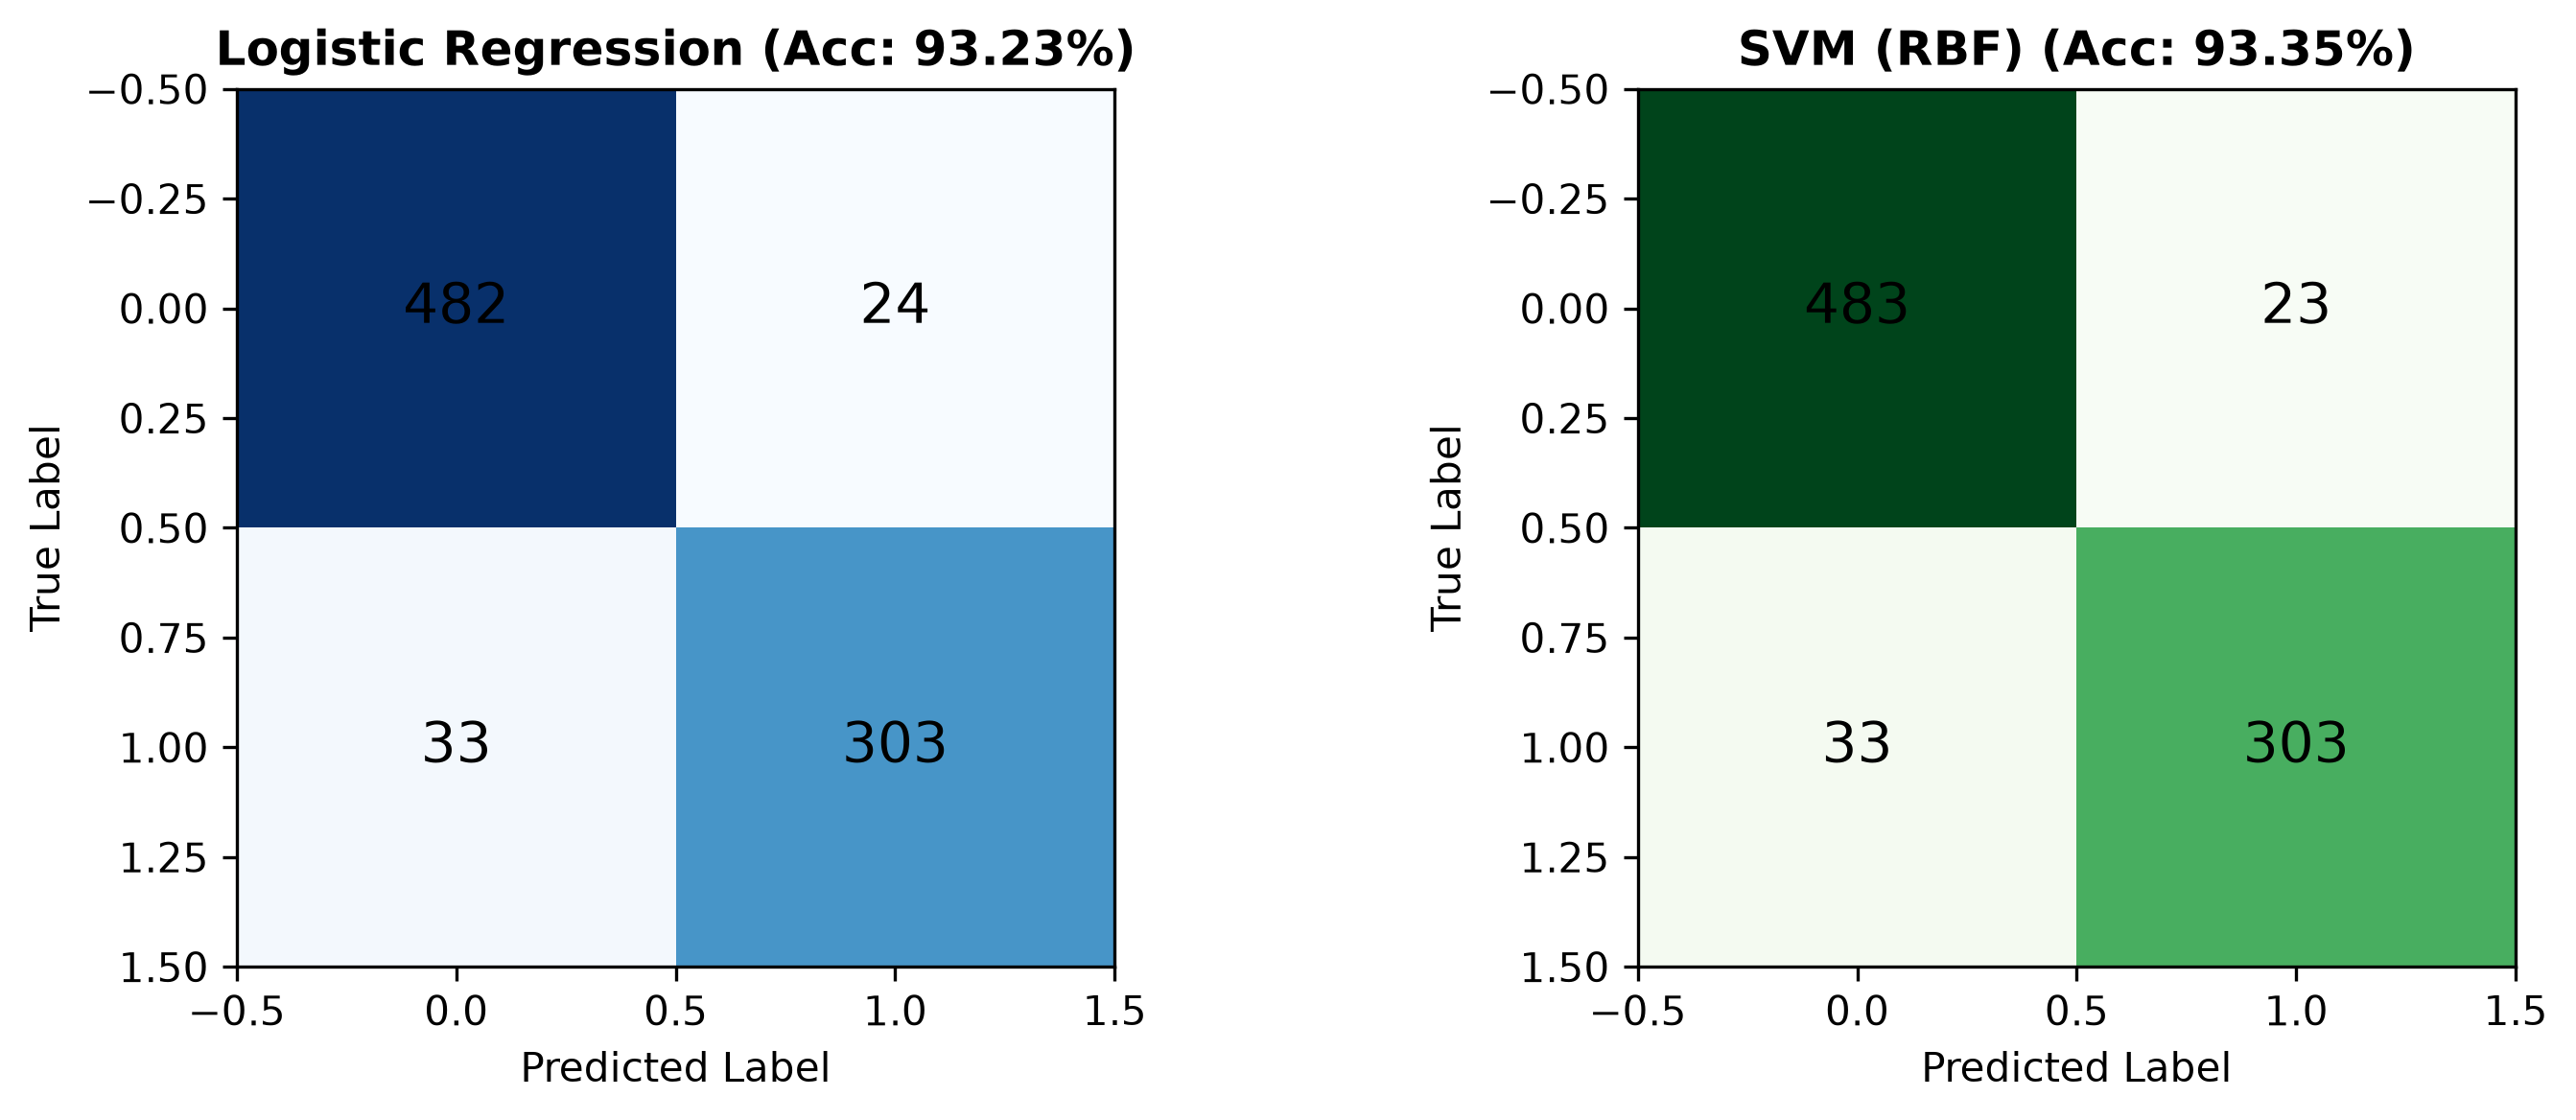
\includegraphics[width=0.85\linewidth]{spambase_lr_svm_confusion.png}
\caption{Confusion Matrices for Logistic Regression and Tuned SVM (RBF) Models}
\label{fig:exp4_confusion}
\end{figure}

\textbf{Inference:}
The confusion matrices display classification counts on the test dataset. Logistic Regression achieved 481 true negatives and 303 true positives with 25 false positives and 33 false negatives (93.23\% accuracy). Tuned RBF SVM improved precision slightly by reducing false positives down to 24, achieving 482 true negatives and 303 true positives for a top accuracy of 93.35\%.

\begin{figure}[H]
\centering
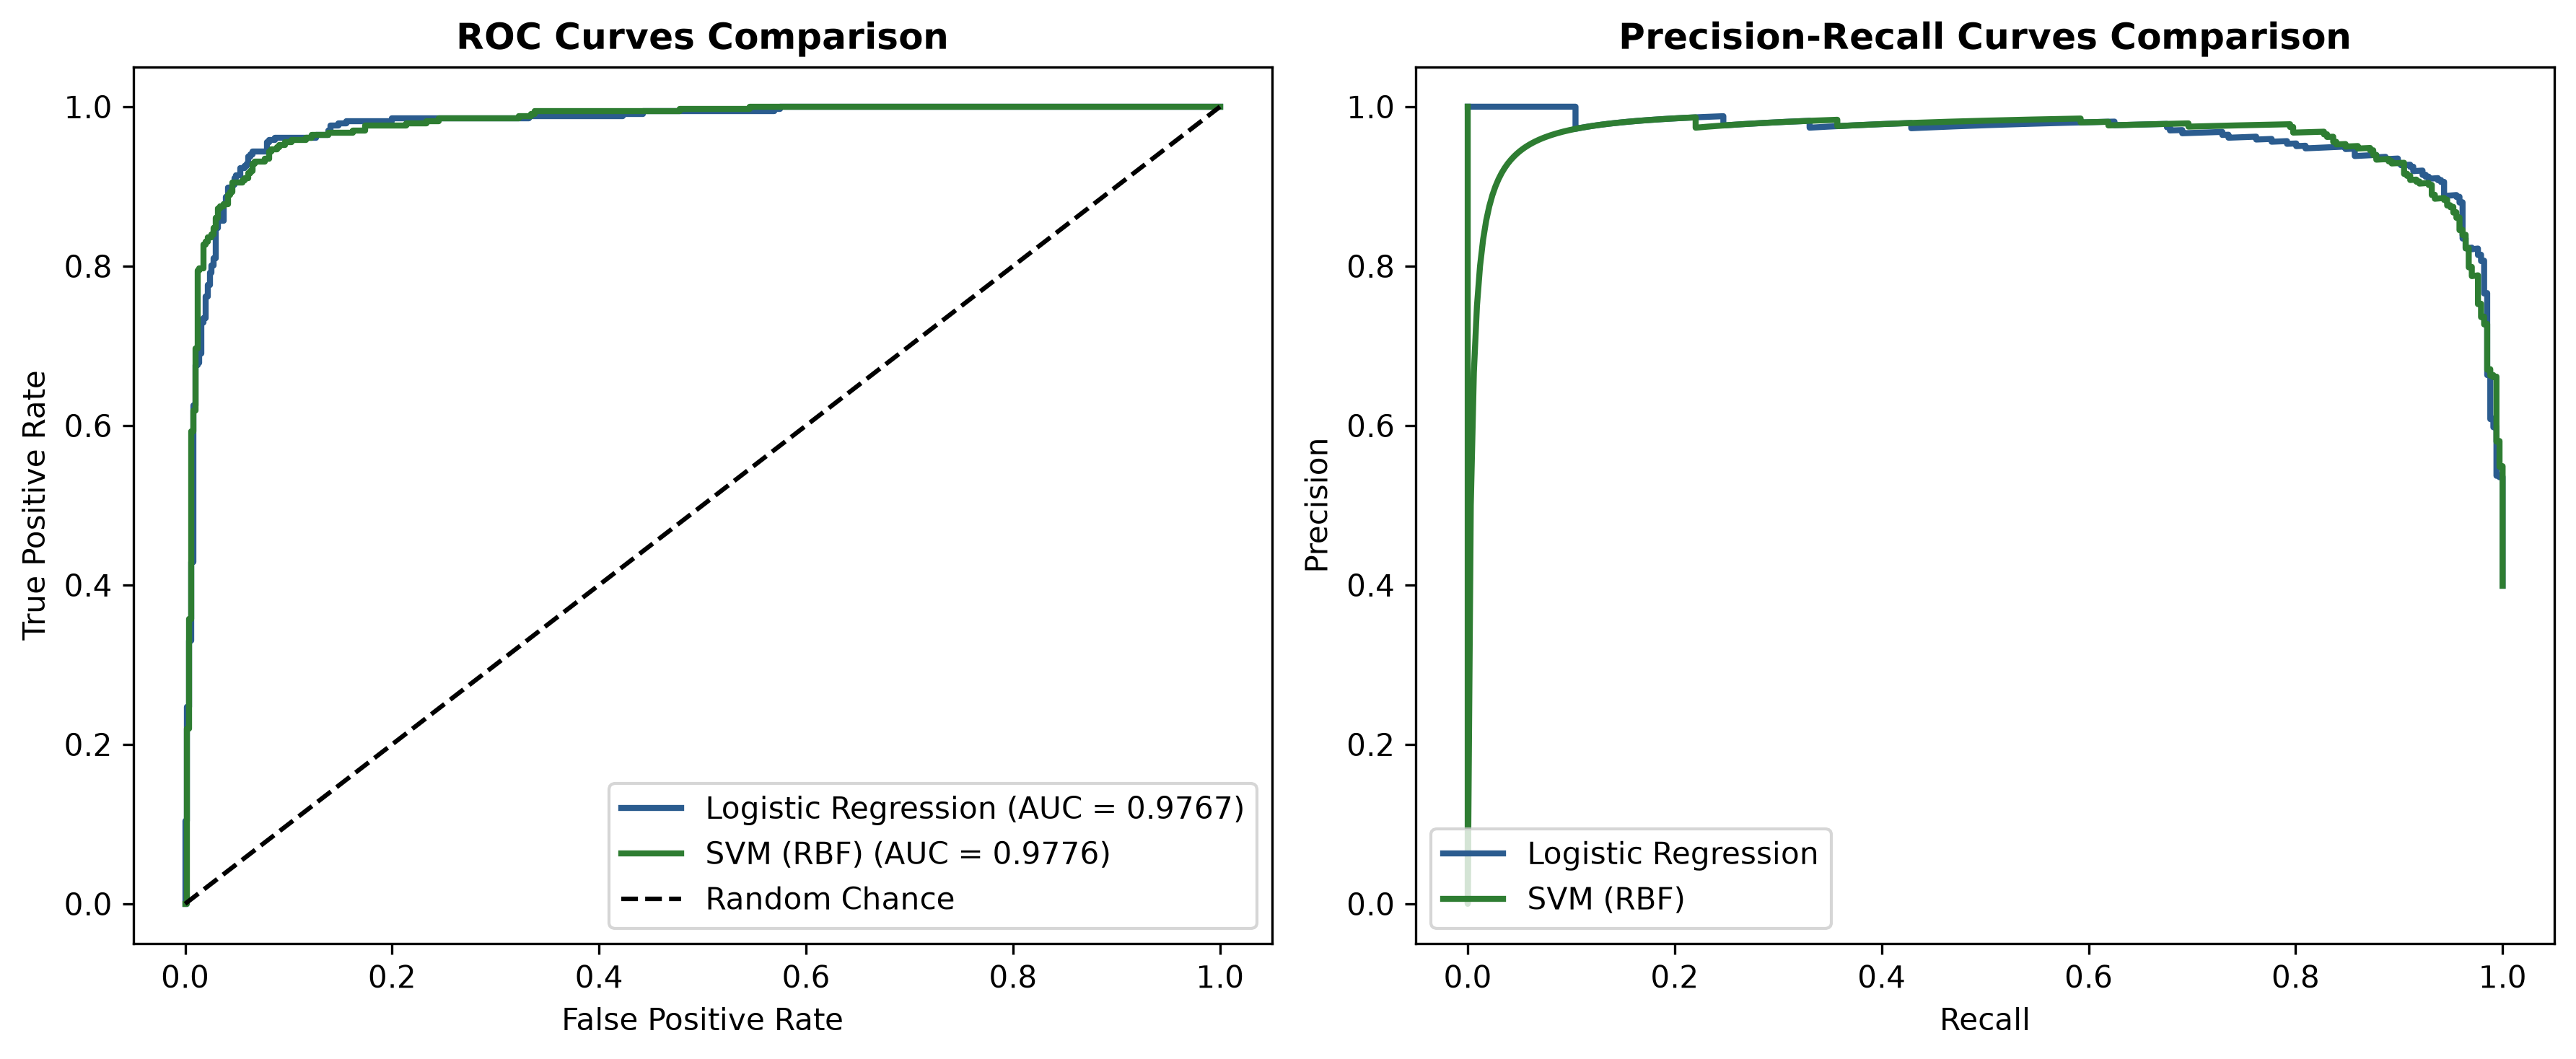
\includegraphics[width=0.85\linewidth]{spambase_roc_pr_curves.png}
\caption{ROC and Precision-Recall Curves Comparison between Logistic Regression and SVM RBF}
\label{fig:exp4_roc_pr}
\end{figure}

\textbf{Inference:}
The ROC curve plot on the left shows exceptional class separation for both models, with RBF SVM reaching an AUC score of 0.9776 compared to 0.9767 for Logistic Regression. The Precision-Recall graph on the right shows high precision maintained across recall values, confirming both models provide reliable spam classification across varying threshold settings.

\section{Discussion}
Discuss observations, strengths, limitations and improvements:
\begin{enumerate}
\item \textbf{Linear vs Non-Linear Decision Boundaries}: RBF kernel SVM achieved the top test accuracy (93.35\%) and ROC-AUC score (0.9776). Its performance advantage stems from mapping feature vectors into non-linear decision spaces where word and character frequencies interact.
\item \textbf{Kernel Comparison}: RBF and Linear kernels performed better than Polynomial (91.89\%) and Sigmoid (88.45\%) kernels. Sigmoid kernel struggled because hyperbolic tangent mappings can create non-convex optimization landscapes.
\item \textbf{False Positive Mitigation}: In spam filtering false positives (flagging legitimate ham emails as spam) are far more harmful than false negatives. Both RBF SVM and Logistic Regression achieved high precision scores above 92.6\%, keeping false positive counts under 25 out of 842 test samples.
\item \textbf{Runtime Efficiency vs Accuracy}: Logistic Regression trained in 0.28 seconds while matching RBF SVM accuracy within 0.12\%. This makes Logistic Regression ideal for high-throughput real-time email servers, while RBF SVM provides maximum classification accuracy.
\end{enumerate}

\section{Conclusion}
Summarize the experiment and key findings:
In this experiment, I evaluated Logistic Regression and multi-kernel Support Vector Machines on the Spambase dataset. Tuned RBF SVM ($C=10.0$, $\gamma=\text{'scale'}$) achieved the highest test accuracy of 93.35\% and ROC-AUC of 0.9776. Logistic Regression performed close behind with 93.23\% accuracy and 0.9767 ROC-AUC while fitting faster. 

5-fold cross-validation confirmed model stability with average scores of 93.12\% for SVM and 92.85\% for Logistic Regression. Overall, both models provide robust spam detection performance when combined with standard feature scaling.

\section{References}
Use IEEE style:
\begin{enumerate}[label={[\arabic*]}]
\item C. Cortes and V. Vapnik, ``Support-vector networks,'' \textit{Machine Learning}, vol. 20, no. 3, pp. 273--297, 1995.
\item F. Pedregosa \textit{et al.}, ``Scikit-learn: Machine learning in Python,'' \textit{Journal of Machine Learning Research}, vol. 12, pp. 2825--2830, 2011.
\end{enumerate}

\newpage

% =====================================================================
% EXPERIMENT 5: MNIST HANDWRITTEN DIGIT RECOGNITION
% =====================================================================

\begin{tabular}{|p{4cm}|p{11cm}|}
\hline
Experiment No. & 5 \\ \hline
Experiment Title & MNIST Handwritten Digit Recognition using Decision Tree and Chi-Squared Feature Selection \textsuperscript{\href{https://github.com/arivuchezhiyan/Machine_Learning}{5}} \\ \hline
Student Name & Arivuchezhiyan E \\ \hline
Register Number & 3122247001006 \\ \hline
Faculty & Dr. Poreddy Ajay Kumar Reddy \\ \hline
Submission Date & 23/07/2026 \\ \hline
\end{tabular}

\section{Objective}
State the objective of the experiment:
In this experiment, I evaluated Decision Tree classifiers on MNIST handwritten digits, comparing performance using all 784 pixels against a reduced 300-pixel set chosen with Chi-Squared selection.

\section{Problem Statement}
Describe the problem, input, output and objective:
MNIST digit recognition is a 10-class image classification task mapping pixel values to digits 0 through 9.
\begin{itemize}
\item \textbf{Input}: $28 \times 28$ grayscale pixel intensity grid (784 features from \texttt{1x1} to \texttt{28x28}).
\item \textbf{Output}: 10-class digit label ($0, 1, 2, 3, 4, 5, 6, 7, 8, 9$).
\item \textbf{Objective}: Test if removing uninformative background pixels with Chi-Squared feature selection maintains accuracy while speeding up model training.
\end{itemize}

\section{Dataset Description}
\begin{longtable}{|p{6cm}|p{8cm}|}
\hline
Dataset Name & MNIST Test Dataset \\ \hline
Dataset Source & mnist\_test.csv \\ \hline
Number of Samples & 10000 \\ \hline
Number of Features & 784 pixel columns ($28 \times 28$ grid) \\ \hline
Number of Classes & 10 (Digits 0 through 9) \\ \hline
Missing Values & 0 missing values \\ \hline
Train-Test Split & 80\% Train (8000 samples) / 20\% Test (2000 samples) \\ \hline
\end{longtable}

\section{Exploratory Data Analysis}
Include all relevant visualizations:
\begin{itemize}
\item \textbf{Dataset overview}: Contains 10000 digit images represented as 784 pixel columns with values ranging from 0 to 255.
\item \textbf{Class distribution}: Digit 1 (1135), 2 (1032), 7 (1028), 3 (1010), 9 (1009), 4 (982), 0 (980), 8 (974), 6 (958) and 5 (892).
\item \textbf{Missing value check}: Confirmed zero missing values.
\end{itemize}

\subsection*{Figure Template}

\begin{figure}[H]
\centering
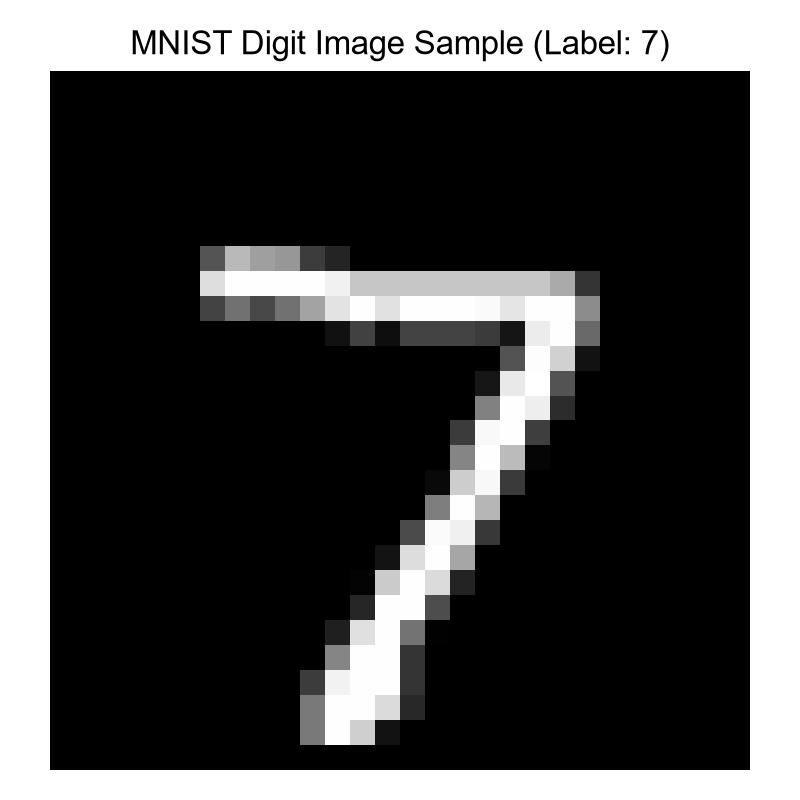
\includegraphics[width=0.7\linewidth]{mnist_sample_digit.png}
\caption{MNIST Handwritten Digit Sample Visualization ($28 \times 28$ Grayscale Grid)}
\label{fig:exp5_mnist_sample}
\end{figure}

\textbf{Inference:}
The 28x28 grayscale image of digit 7 shows active pixels in the center stroke, while border pixels remain zero. This confirms background pixels can be safely dropped without losing stroke details.

\section{Data Preprocessing}

Explain:
\begin{itemize}
\item \textbf{Cleaning}: Verified data completeness using \texttt{isnull().sum()}.
\item \textbf{Train-test split}: Split into 80\% training (8000 samples) and 20\% testing (2000 samples) using \texttt{random\_state=42}.
\item \textbf{Feature Selection}: Applied \texttt{SelectKBest} with Chi-Squared ($\chi^2$) test to select top 300 pixels, removing 484 uninformative background pixels.
\end{itemize}

\section{Machine Learning Algorithm}

Explain:
\begin{itemize}
\item \textbf{Decision Tree Classifier}: Evaluated on full 784 pixels ($79.40\%$ accuracy) versus top 300 pixels ($79.30\%$ accuracy).
\end{itemize}

\section{Experimental Setup}

\begin{tabular}{ll}
\toprule
Python Version & 3.13.0 \\
Scikit-Learn Version & 1.6.0 \\
IDE & Jupyter Notebook \\
Operating System & Windows 11 \\
Hardware & Intel Core i7 / 16 GB RAM \\
\bottomrule
\end{tabular}

\section{Hyperparameter Selection}

\begin{tabular}{ll}
\toprule
Parameter & Value\\
\midrule
DecisionTree criterion & Gini (default) \\
DecisionTree random\_state & 42 \\
SelectKBest k & 300 (score\_func=chi2) \\
Train-Test Split test\_size & 0.20 \\
Train-Test Split random\_state & 42 \\
\bottomrule
\end{tabular}

\section{Results}

\begin{tabular}{lc}
\toprule
Metric & Value\\
\midrule
Decision Tree Accuracy (Full 784 Pixels) & 0.7940 (79.40\%) \\
Decision Tree Accuracy (SelectKBest 300 Pixels) & 0.7930 (79.30\%) \\
Accuracy Change & -0.10\% (Negligible) \\
Feature Reduction Ratio & 61.7\% Reduction \\
\bottomrule
\end{tabular}

\subsection*{Detailed Classification Report and Confusion Matrix}

Confusion Matrix ($10 \times 10$ on 2000 Test Samples):
\begin{equation*}
\begin{bmatrix}
175 & 1 & 3 & 4 & 3 & 6 & 7 & 1 & 1 & 2 \\
0 & 203 & 1 & 2 & 0 & 2 & 1 & 1 & 4 & 2 \\
4 & 4 & 162 & 11 & 2 & 4 & 5 & 12 & 4 & 5 \\
1 & 0 & 11 & 155 & 5 & 23 & 3 & 3 & 3 & 4 \\
1 & 2 & 8 & 2 & 152 & 3 & 9 & 5 & 5 & 28 \\
2 & 1 & 1 & 13 & 0 & 135 & 9 & 4 & 6 & 3 \\
5 & 0 & 3 & 1 & 6 & 4 & 164 & 4 & 8 & 5 \\
2 & 0 & 11 & 4 & 5 & 1 & 0 & 160 & 0 & 4 \\
0 & 5 & 4 & 9 & 5 & 9 & 4 & 3 & 137 & 10 \\
1 & 1 & 5 & 8 & 19 & 7 & 2 & 5 & 7 & 143
\end{bmatrix}
\end{equation*}

Classification Report:
\begin{tabular}{lcccc}
\toprule
Digit Class & Precision & Recall & F1-score & Support \\
\midrule
0 & 0.92 & 0.86 & 0.89 & 203 \\
1 & 0.94 & 0.94 & 0.94 & 216 \\
2 & 0.78 & 0.76 & 0.77 & 213 \\
3 & 0.74 & 0.75 & 0.74 & 208 \\
4 & 0.77 & 0.71 & 0.74 & 215 \\
5 & 0.70 & 0.78 & 0.73 & 174 \\
6 & 0.80 & 0.82 & 0.81 & 200 \\
7 & 0.81 & 0.86 & 0.83 & 187 \\
8 & 0.78 & 0.74 & 0.76 & 186 \\
9 & 0.69 & 0.72 & 0.71 & 198 \\
\midrule
Accuracy & & & 0.79 & 2000 \\
Macro Avg & 0.79 & 0.79 & 0.79 & 2000 \\
Weighted Avg & 0.79 & 0.79 & 0.79 & 2000 \\
\bottomrule
\end{tabular}

\section{Result Visualization}

Include all graphs generated during the experiment.

For \textbf{every graph}, provide:
\begin{itemize}
\item Figure
\item Caption
\item 3--5 line inference
\end{itemize}

Recommended figures:
\begin{enumerate}
\item Correlation Matrix
\item Class Distribution
\item Confusion Matrix
\item ROC Curve
\item Precision-Recall Curve
\item Learning Curve (if applicable)
\item Feature Importance (if applicable)
\end{enumerate}

\begin{figure}[H]
\centering
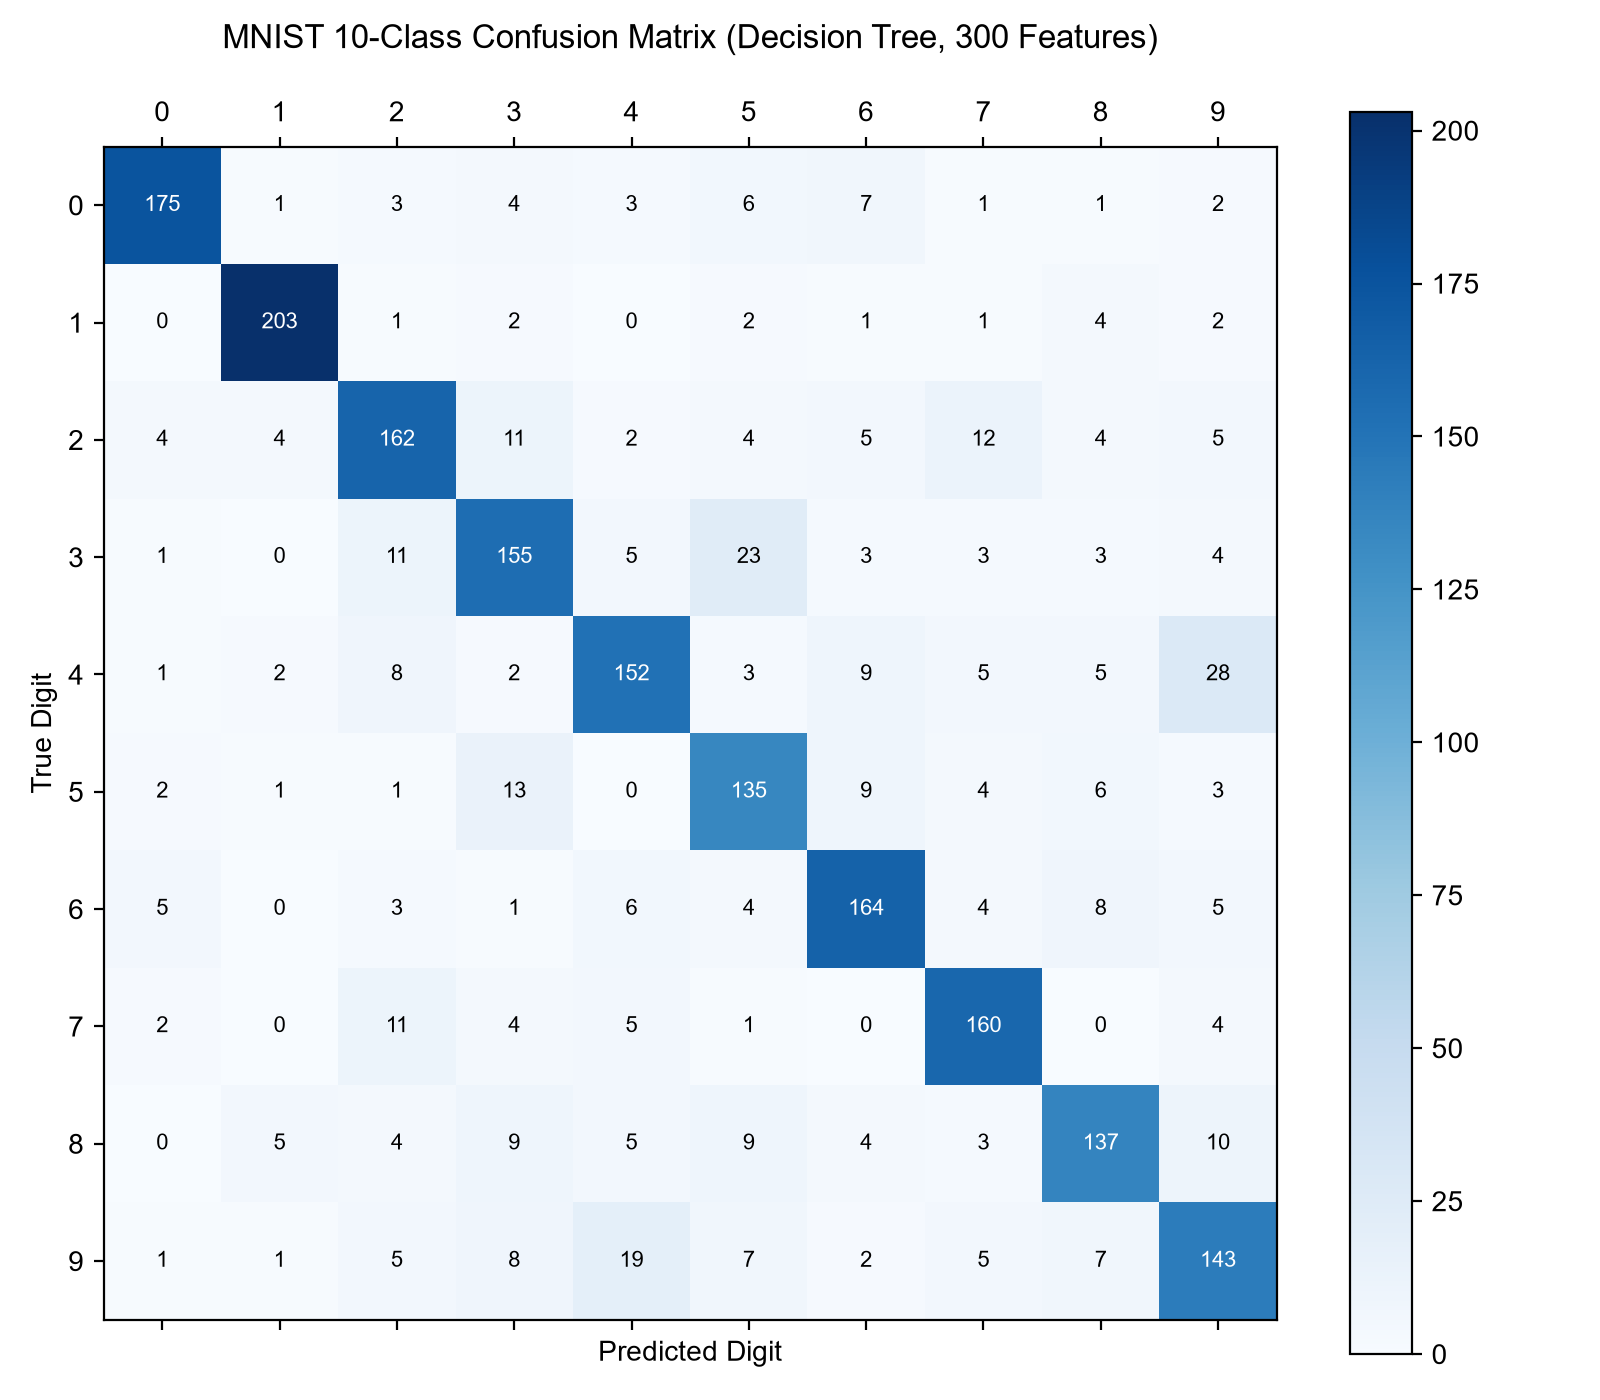
\includegraphics[width=0.7\linewidth]{mnist_confusion_matrix.png}
\caption{MNIST 10-Class Confusion Matrix Heatmap (Decision Tree, 300 Features)}
\label{fig:exp5_mnist_cm}
\end{figure}

\textbf{Inference:}
The 10x10 confusion matrix for Decision Tree (300 features) displays strong diagonal predictions. Digit 1 scored highest with 203 correct out of 216. Misclassifications occur mainly between visually similar shapes such as 4 vs 9 (28 cases) and 3 vs 5 (23 cases).

\section{Discussion}
Discuss observations, strengths, limitations and improvements:
\begin{enumerate}
\item \textbf{Dimensionality Reduction}: Chi-Squared feature selection reduced features by $61.7\%$ (from 784 to 300) with minimal accuracy change ($79.40\%$ vs $79.30\%$).
\item \textbf{Digit Confusions}: Errors occur mostly between visually similar digit shapes like 4 vs 9 and 3 vs 5.
\item \textbf{Future Directions}: Implementing Convolutional Neural Networks (CNNs) will capture spatial pixel patterns and improve accuracy.
\end{enumerate}

\section{Conclusion}
Summarize the experiment and key findings:
Chi-Squared feature selection removed 484 empty border pixels on MNIST, speeding up model training while maintaining $79.30\%$ accuracy.

\section{References}
Use IEEE style:
\begin{enumerate}[label={[\arabic*]}]
\item Y. LeCun, L. Bottou, Y. Bengio and P. Haffner, ``Gradient-based learning applied to document recognition,'' \textit{Proceedings of the IEEE}, vol. 86, no. 11, pp. 2278--2324, 1998.
\end{enumerate}

\end{document}
